\chapter{Numele aplicației}

\chapter{Colectarea cerințelor}

În cadrul acestui capitol sunt detaliate funcționalitățile sistemului Neuro-Guardian, interacțiunile dintre utilizatori și platformă, precum și constrângerile tehnice sub care funcționează soluția propusă.

\section{Actorii sistemului}

Actorii reprezintă entitățile externe care interacționează cu sistemul. În cadrul platformei Neuro-Guardian, am identificat următoarele categorii:

\begin{itemize}
    \item \textbf{Angajat Spital:} Actorul generic care include funcționalitățile de bază de autentificare (Înregistrare, Autentificare, Deconectare).
    \item \textbf{Administrator:} Moștenește trăsăturile angajatului și are responsabilitatea gestionării fluxului administrativ al pacienților (internări, externări și alocarea resurselor/paturilor).
    \item \textbf{Doctor:} Actorul principal în procesul de îngrijire, responsabil de preluarea pacienților și monitorizarea stării lor clinice și emoționale în timp real.
    \item \textbf{Camera Web (Sistem Extern):} Furnizează fluxul de date video necesar procesului de captare a cadrelor.
    \item \textbf{CSNN - Convolutional Spiking Neural Network (Sistem Extern):} Modelul de inteligență artificială care procesează cadrele recepționate și returnează predicțiile emoționale.
\end{itemize}

\section{Diagrama cazurilor de utilizare}

Diagrama cazurilor de utilizare, prezentată în Figura \ref{fig:diagrama_uml}, oferă o imagine de ansamblu asupra modului în care funcționalitățile sunt distribuite între actori.

\begin{figure}[htbp]
    \centering
    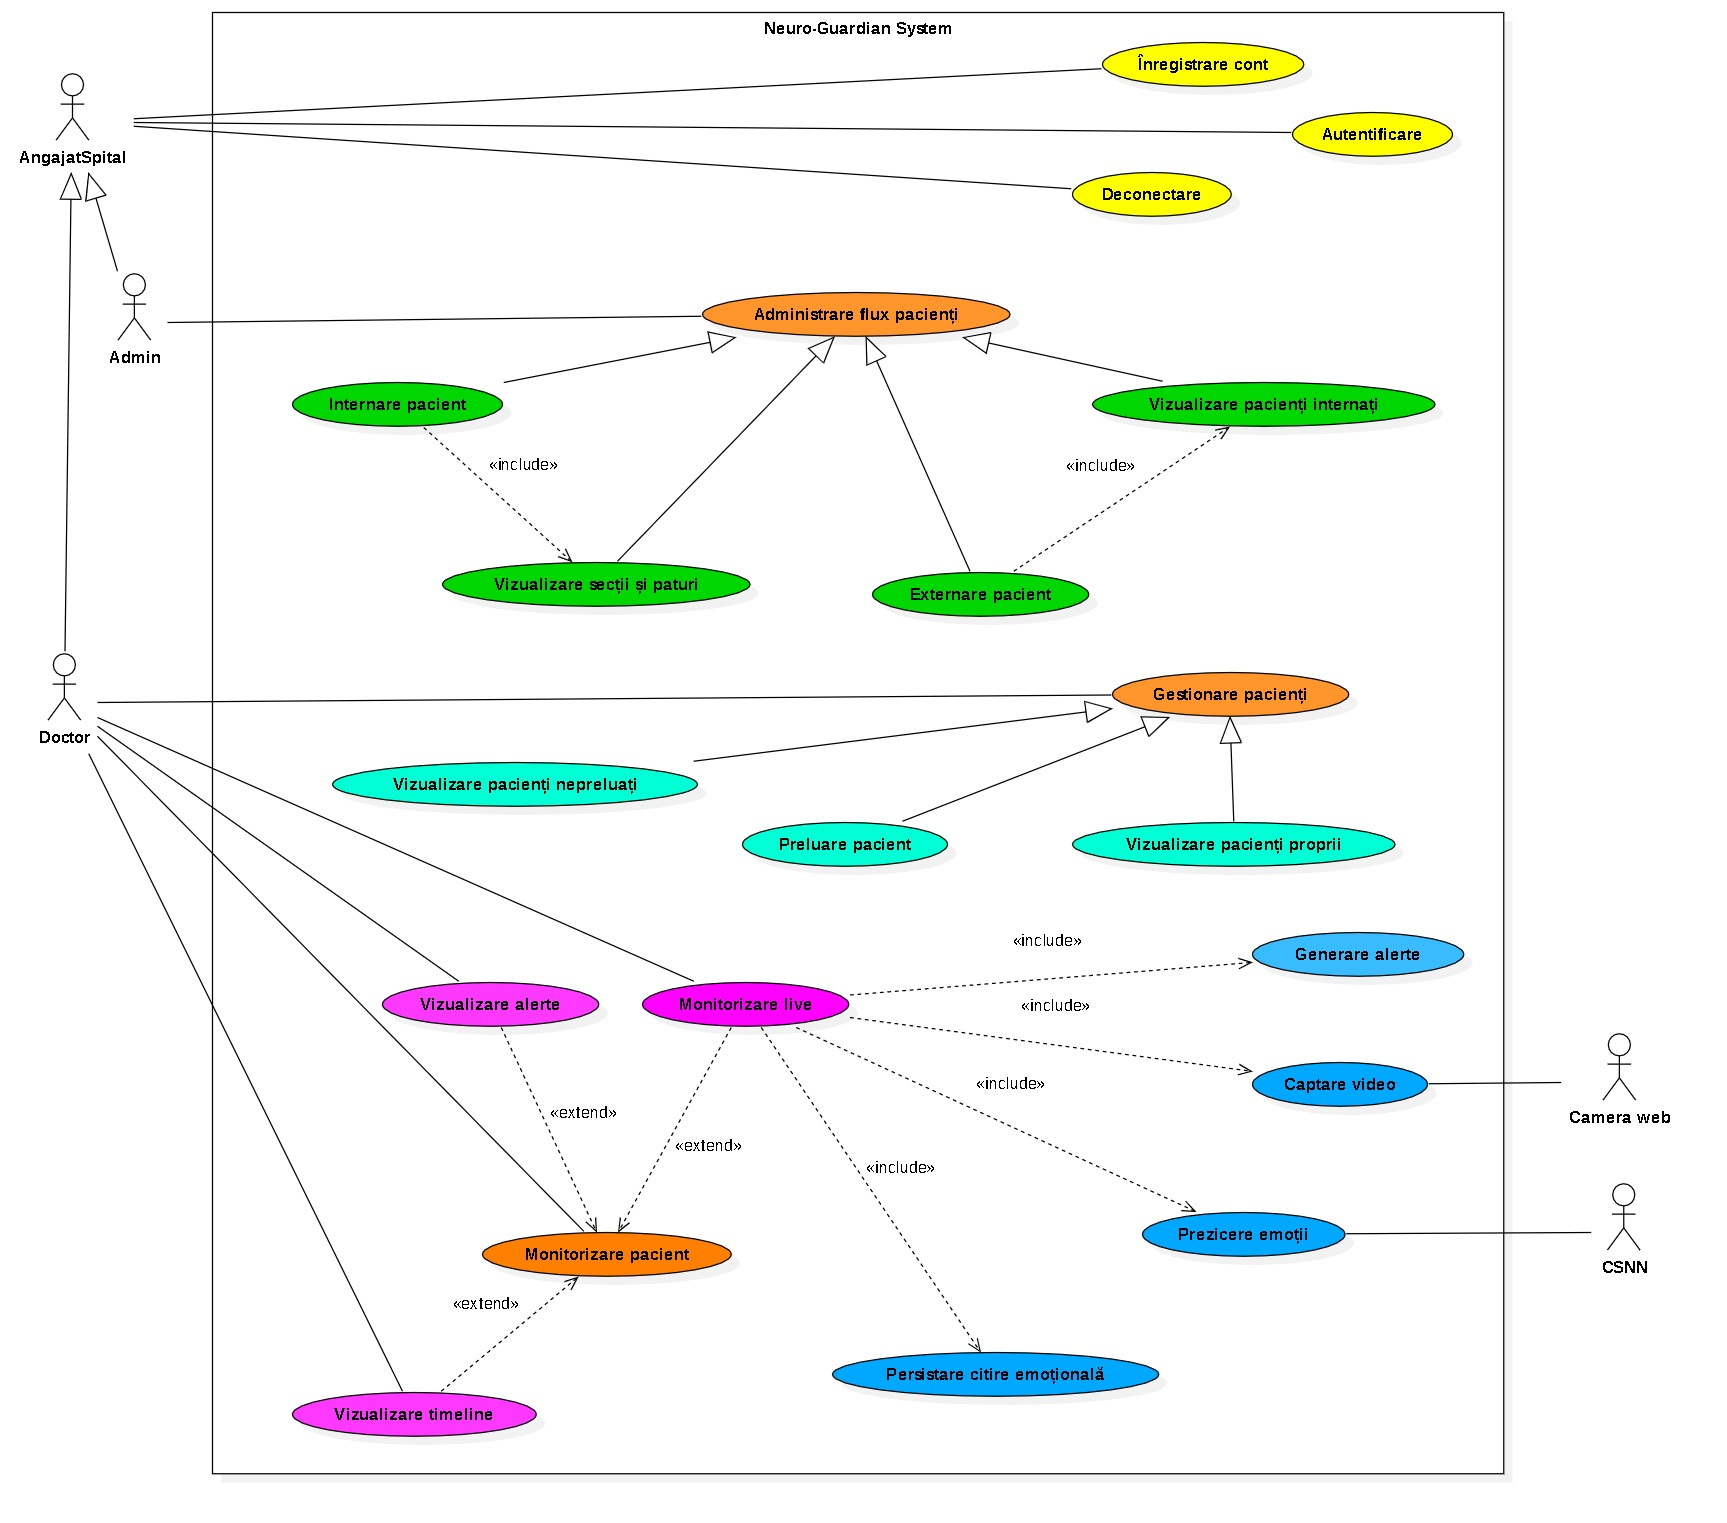
\includegraphics[width=0.83\textwidth]{figures/diagrams/UseCaseDiagram.jpg}
    \caption{Diagrama cazurilor de utilizare - Sistemul Neuro-Guardian}
    \label{fig:diagrama_uml}
\end{figure}

\section{Descrierea detaliată a unui caz de utilizare}

În această secțiune este detaliat fluxul principal de interacțiune pentru cazul de utilizare \textbf{Gestionare Pacienți}, reprezentat grafic în Figura \ref{fig:diagrama_uml}. Acest caz de utilizare este central pentru activitatea clinică a medicului, asigurând tranziția între selecția pacienților și monitorizarea activă.

\begin{table}[htbp]
\centering
\small
\begin{tabularx}{\textwidth}{|l|X|}
\hline
\rowcolor[HTML]{EFEFEF} 
\multicolumn{2}{|l|}{\textbf{Elemente de identificare}} \\ \hline
\textbf{Nume} & Gestionare pacienți \\ \hline
\textbf{Actori} & Doctor \\ \hline
\textbf{Descriere} & Procesul prin care un medic vizualizează lista pacienților din secție, preia responsabilitatea pentru un pacient nou sau comută între pacienții deja asignați pentru a vizualiza datele biometrice și emoționale. \\ \hline

\rowcolor[HTML]{EFEFEF} 
\multicolumn{2}{|l|}{\textbf{Condiții de context}} \\ \hline
\textbf{Precondiții} & 1. Medicul este autentificat în sistem. \newline 2. Pacienții sunt deja internați în secție (via Admin). \newline 3. Conexiunea WebSocket cu modelul AI este activă. \\ \hline
\textbf{Postcondiții} & Interfața reflectă starea în timp real a pacientului selectat, iar baza de date actualizează relația medic-pacient. \\ \hline

\rowcolor[HTML]{EFEFEF} 
\multicolumn{2}{|l|}{\textbf{Scenariu Principal de Succes (MSS)}} \\ \hline
\textbf{Flux normal} & 
1. Medicul accesează dashboard-ul; sistemul afișează implicit datele ultimului pacient preluat. \newline
2. Medicul acționează butonul „Show panel” pentru a extinde panoul de selecție. \newline
3. Sistemul interoghează baza de date și afișează două liste: „Available Patients” și „My Patients”. \newline
4. Medicul identifică un pacient nepreluat și selectează opțiunea „Take patient”. \newline
5. Sistemul realizează maparea medic-pacient și trimite medicul către pagina destinată pacientului respectiv\newline
6. Medicul selectează un alt pacient din lista „My Patients” pentru a verifica evoluția acestuia. \newline
7. Sistemul comută contextul de monitorizare, afișând informațiile specifice noului pacient selectat. \newline
8. Medicul acționează „Hide panel” pentru a maximiza spațiul de vizualizare a detaliilor pacientului. \newline
9. Sistemul ascunde panoul lateral și trece în modul de monitorizare imersivă. \\ \hline

\rowcolor[HTML]{EFEFEF} 
\multicolumn{2}{|l|}{\textbf{Scenarii alternative}} \\ \hline
\textbf{Alt. 1} & \textbf{Medicul nu are pacienți în responsabilitate:} \newline
1a. Sistemul afișează un mesaj de informare și prezintă doar lista pacienților nepreluați. \newline
1b. Medicul efectuează preluarea primului pacient (se revine la pasul 5 din MSS). \\ \hline
\textbf{Alt. 2} & \textbf{Inexistența pacienților nepreluați:} \newline
3a. Lista „Available patients” apare goală; medicul poate gestiona doar portofoliul actual de pacienți (se revine la pasul 6 din MSS). \\ \hline

\rowcolor[HTML]{EFEFEF} 
\multicolumn{1}{|l|}{\textbf{Excepții}} \\ \hline
\textbf{Excepție 1} & \textbf{Pacientul este externat simultan:} Sistemul blochează preluarea și notifică medicul că datele nu mai sunt disponibile. \\ \hline

\rowcolor[HTML]{EFEFEF} 
\multicolumn{2}{|l|}{\textbf{Cerințe de calitate}} \\ \hline
\textbf{Performanță} & Timpul de comutare între doi pacienți nu trebuie să depășească 1 secundă pentru datele textuale. \\ \hline
\textbf{Fiabilitate} & Persistarea asocierii medic-pacient trebuie să fie confirmată tranzacțional în baza de date. \\ \hline
\end{tabularx}
\caption{Descrierea detaliată a scenariului de utilizare: Gestionare pacienți}
\label{tab:detaliu_gestiune}
\end{table}

\section{Cerințe nefuncționale (NFR)}

Cerințele nefuncționale definesc criteriile de calitate și constrângerile tehnice ale sistemului.

\subsection{Securitate și control acces}
\begin{itemize}
    \item \textbf{NFR-S1:} Toate operațiile sensibile necesită autentificare pe bază de Bearer JWT.
    \item \textbf{NFR-S2:} Autorizare strictă pe rol (ADMIN vs DOCTOR); medicii pot vizualiza doar pacienții care le sunt asignați.
    \item \textbf{NFR-S3:} Parolele sunt stocate exclusiv în format hashed folosind algoritmul \textit{bcrypt}.
    \item \textbf{NFR-S4:} Token-urile au timp de expirare implementat, iar refresh token-urile sunt rotite automat și invalidate la logout.
    \item \textbf{NFR-S5:} Validarea riguroasă a input-ului la frontierele API (câmpuri obligatorii, formate de timestamp valide).
\end{itemize}

\subsection{Confidențialitate și protecția datelor}
\begin{itemize}
    \item \textbf{NFR-P1:} Datele pacienților sunt accesibile doar personalului medical autorizat direct.
    \item \textbf{NFR-P2:} Minimizarea expunerii datelor; sistemul nu afișează informații care nu sunt necesare contextului clinic curent.
    \item \textbf{NFR-P3:} Comunicația între client și server se realizează prin protocoale criptate HTTPS/WSS (TLS).
\end{itemize}

\subsection{Performanță și timp real}
\begin{itemize}
    \item \textbf{NFR-F1:} Afișarea emoțiilor se realizează aproape în timp real prin WebSocket, cu o latență minimă, în timp ce persistarea în baza de date se face periodic.
    \item \textbf{NFR-F2:} Limitarea backlog-ului de cadre video procesate pentru a preveni consumul excesiv de memorie RAM pe client.
    \item \textbf{NFR-F3:} Dashboard-ul rămâne responsiv și funcțional chiar și în perioadele de indisponibilitate a motorului de analiză AI.
\end{itemize}

\subsection{Fiabilitate și disponibilitate}
\begin{itemize}
    \item \textbf{NFR-R1:} Mecanism de \textit{fallback}: dacă InfluxDB este indisponibil, sistemul utilizează baza de date principală (Postgres) sau date sintetice pentru continuitate.
    \item \textbf{NFR-R2:} Interfața semnalează vizual deconectarea modelului AI, permițând utilizatorului să continue alte activități administrative.
    \item \textbf{NFR-R3:} Operațiile critice (Check-in/Check-out) sunt tratate tranzacțional pentru a menține consistența între starea patului și cea a pacientului.
\end{itemize}

\subsection{Uzabilitate și Mentenabilitate}
\begin{itemize}
    \item \textbf{NFR-U1:} Interfața oferă feedback vizual clar pentru stările de încărcare sau eroare (Loading/Error states).
    \item \textbf{NFR-M1:} Arhitectură modulară bazată pe TypeScript, cu separare clară între controller, rute și servicii.
    \item \textbf{NFR-M3:} Aplicația este cross-platform (Windows/Linux) utilizând stack-ul Node.js și Vite.
\end{itemize}

\section{Modelul structural}
\label{sec:model-structural}

\subsection{Backend}
\label{subsec:model-structural-backend}

\begin{figure}[htbp]
  \centering

  \begin{subfigure}[t]{0.99\textwidth}
    \centering
    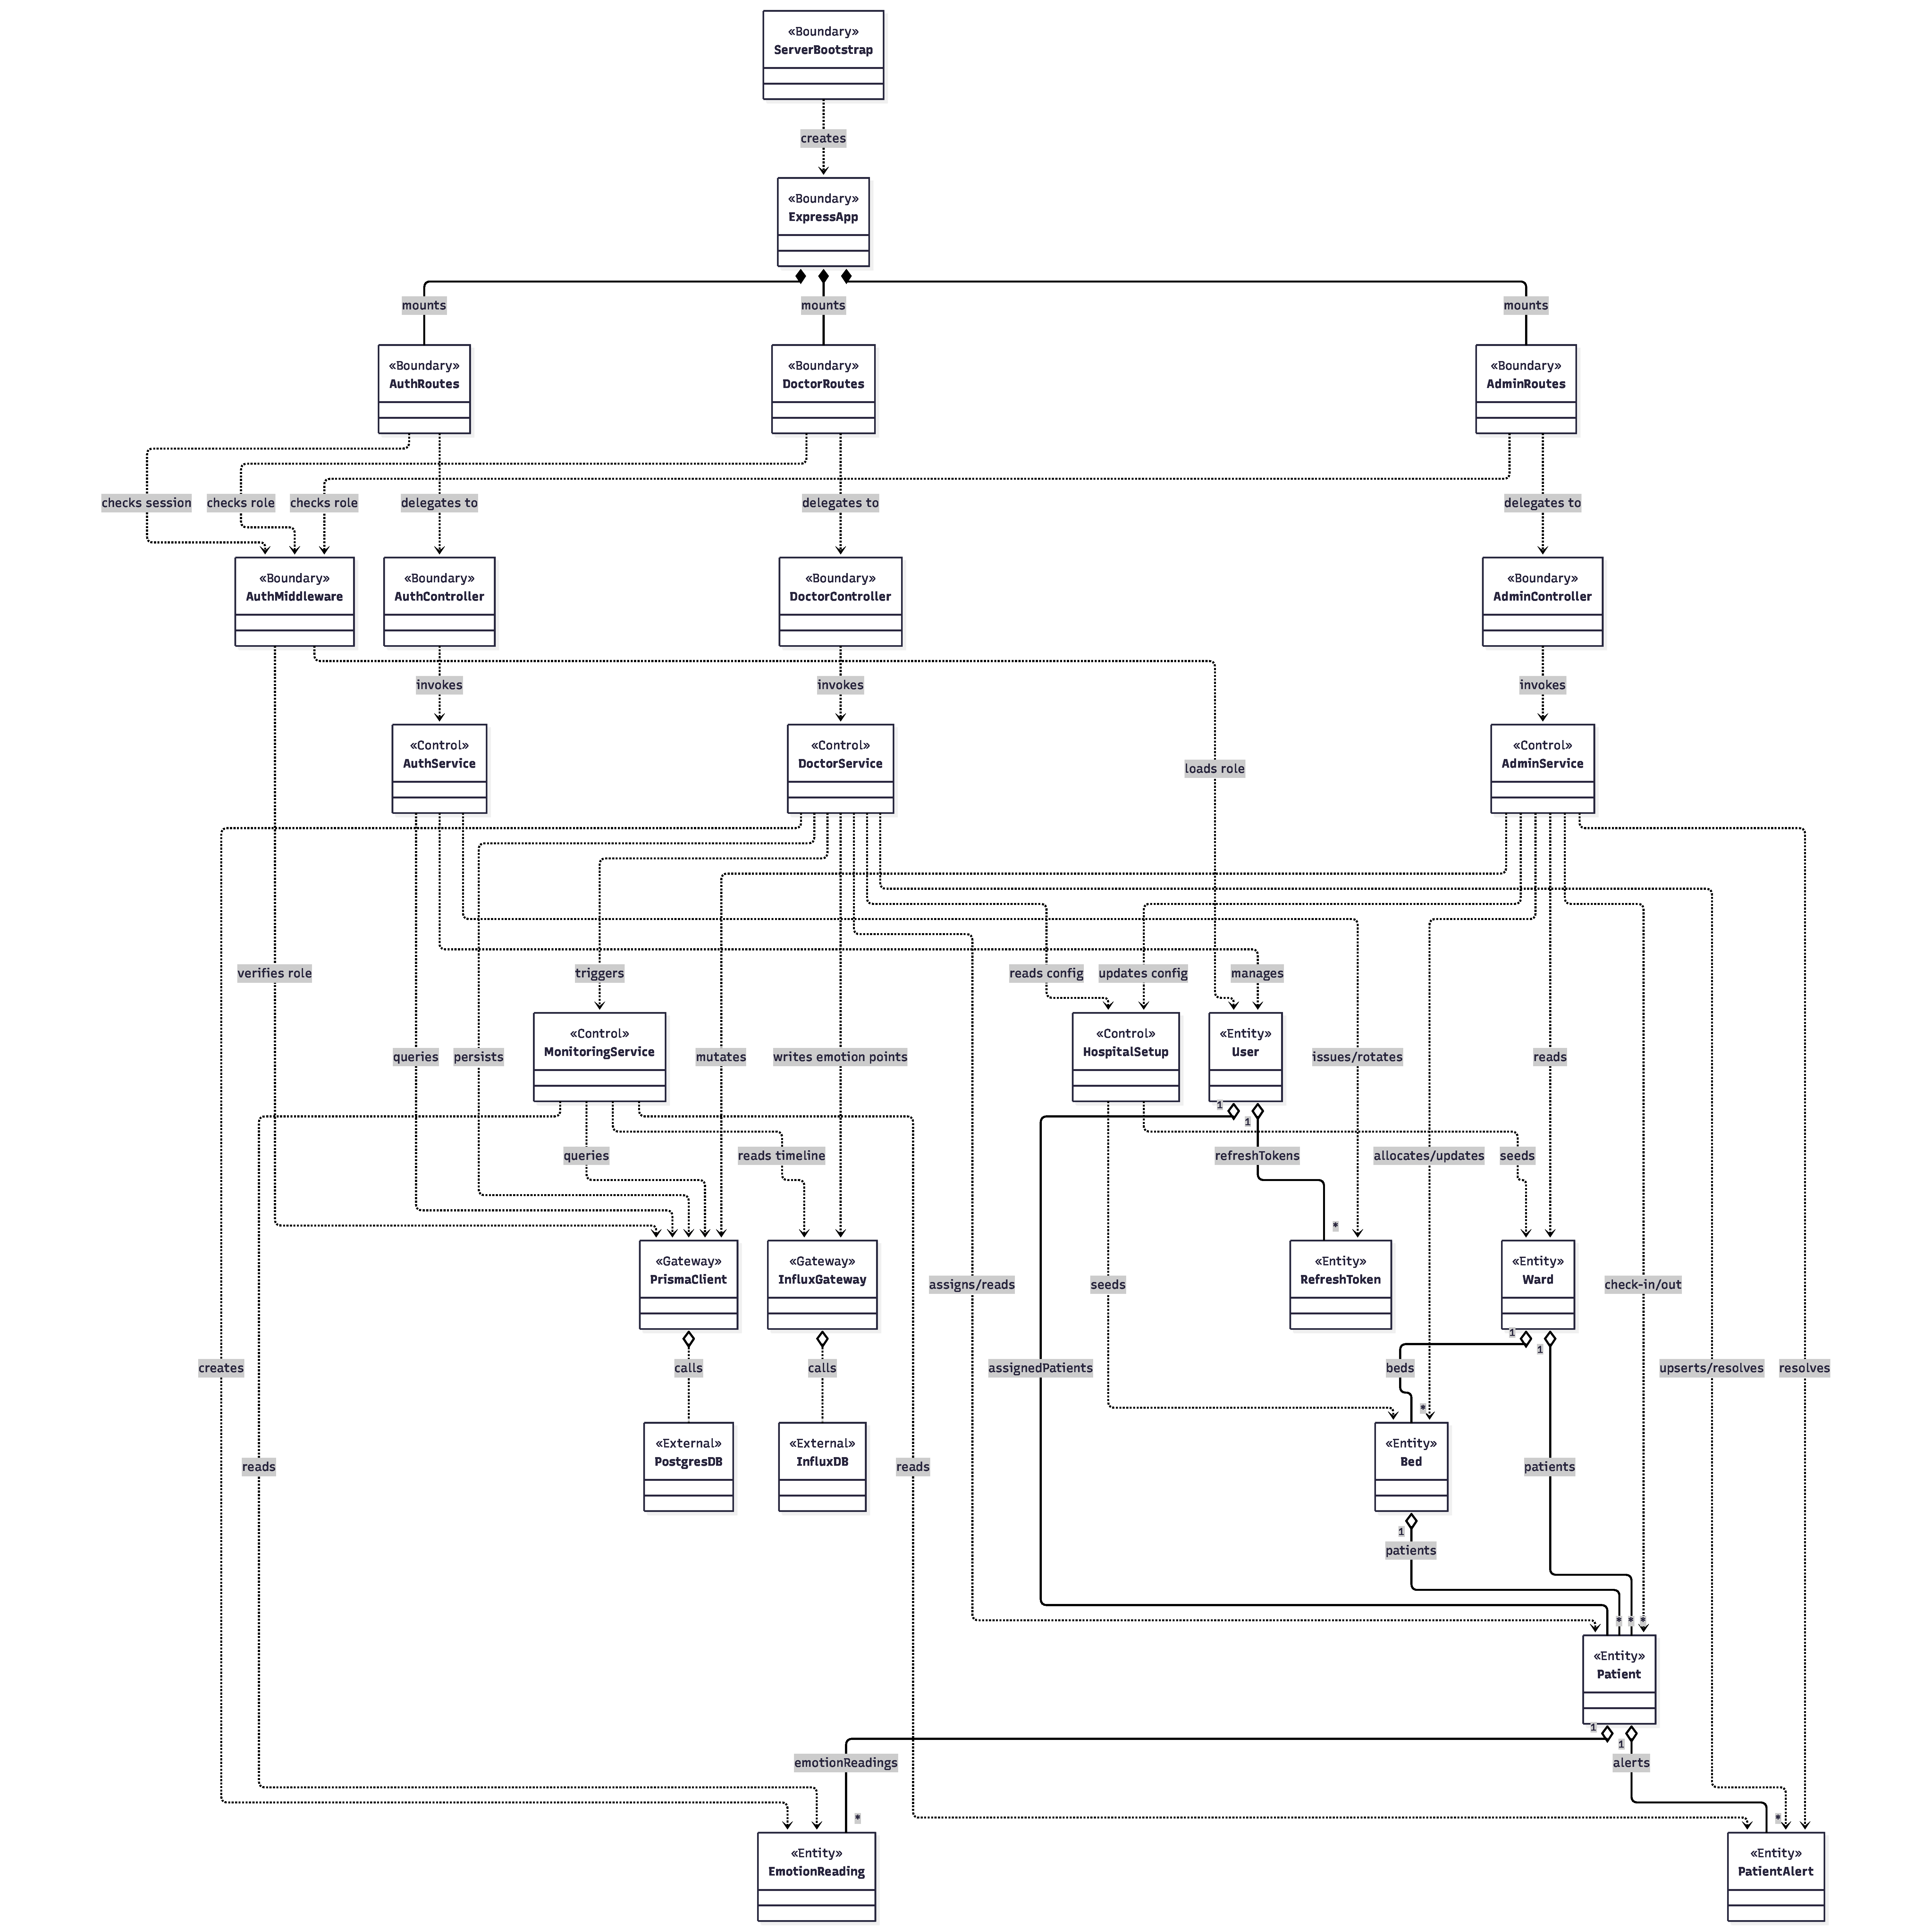
\includegraphics[width=\textwidth]{figures/diagrams/backend-class-diagram-1.pdf}
    \caption{API-ul HTTP: Boundary (Express/Routes/Controllers/Middleware), Control (Services) și persistența prin Gateway/External.}
    \label{fig:backend-ecb-api}
  \end{subfigure}

  \vspace{0.6em}

  \begin{subfigure}[t]{0.99\textwidth}
    \centering
    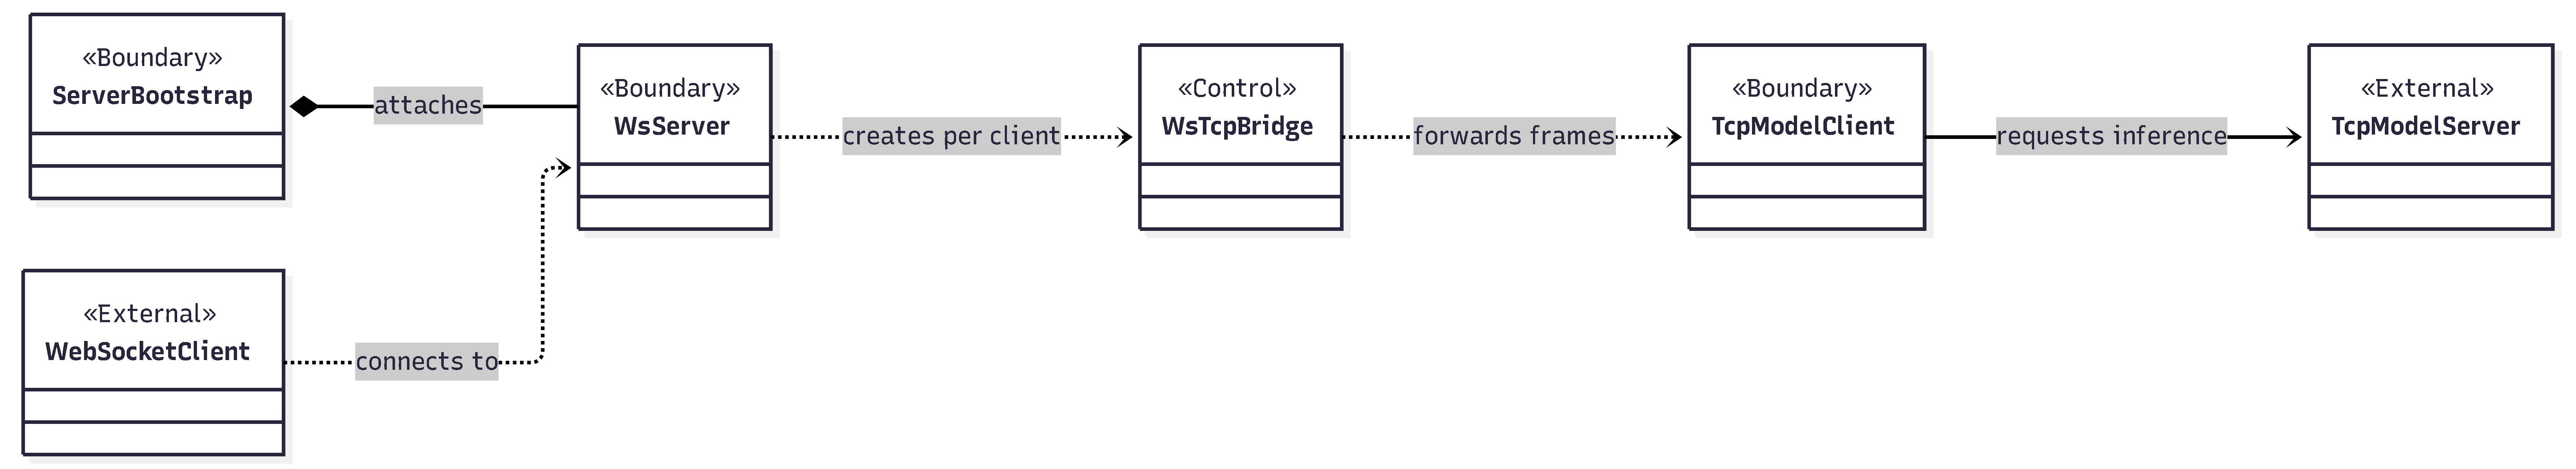
\includegraphics[width=\textwidth]{figures/diagrams/backend-class-diagram-2.png}
    \caption{Canalul de inferență în timp real: WebSocket \texorpdfstring{$\leftrightarrow$}{<->} TCP (model extern).}
    \label{fig:backend-ecb-stream}
  \end{subfigure}

  \caption{Modelul structural al backend-ului, conform ECB (Entity--Control--Boundary) extins cu Gateway și External.}
  \label{fig:backend-ecb}
\end{figure}

Figura~\ref{fig:backend-ecb-api} și Figura~\ref{fig:backend-ecb-stream} ilustrează organizarea backend-ului bazată pe modelul arhitectural \textit{Entity--Control--Boundary} (ECB), structură care asigură o separare clară a responsabilităților:
\begin{itemize}
  \item \textit{Entity} reprezintă nucleul domeniului, adică modelele persistente gestionate în baza de date (ex.: \textit{User}, \textit{Patient}, \textit{EmotionReading}, \textit{PatientAlert}).
  \item \textit{Control} concentrează logica de business și orchestrează fluxurile de lucru (serviciile aplicației).
  \item \textit{Boundary} delimitează interfața către exterior și gestionează comunicarea cu clienții (rute, controllere, middleware, servere de transport).
\end{itemize}

Pentru integrarea cu infrastructura, arhitectura este extinsă cu etichetele \textit{Gateway} și \textit{External}, care izolează accesul la servicii externe și decuplează logica internă de detaliile tehnice (de exemplu, accesul la baze de date). În Figura~\ref{fig:backend-ecb-api}, inițializarea aplicației este realizată de \textit{ServerBootstrap} și \textit{ExpressApp}, care montează rutele (\textit{AuthRoutes}, \textit{DoctorRoutes}, \textit{AdminRoutes}) și aplică \textit{AuthMiddleware} pentru validarea sesiunii și a rolurilor. La nivelul stratului de expunere HTTP, componentele de tip controller (AuthController, DoctorController, AdminController) au fost proiectate conform paradigmei de 'thin controllers' (asigurând o logică minimală de procesare) și deleagă operațiile către servicii (\textit{AuthService}, \textit{DoctorService}, \textit{AdminService}), astfel încât regulile de business și validările specifice domeniului să fie centralizate și ușor de întreținut. Serviciile operează asupra entităților domeniului (de exemplu, \textit{AuthService} gestionează \textit{User}/\textit{RefreshToken}, \textit{DoctorService} gestionează \textit{Patient}/\textit{EmotionReading}/\textit{PatientAlert}, iar \textit{AdminService} gestionează \textit{Ward}/\textit{Bed}/\textit{Patient}).

Persistența și integrarea sunt decuplate prin gateway-uri: \textit{PrismaClient} mediază accesul la baza de date relațională (PostgreSQL), iar \textit{InfluxGateway} asigură scrierea/citirea seriilor temporale în InfluxDB, pentru vizualizări și analiză istorică. Separat de fluxul HTTP, Figura~\ref{fig:backend-ecb-stream} prezintă canalul de procesare în timp real pentru inferență: \textit{WsServer} acceptă conexiuni de la clientul WebSocket al aplicației web, iar \textit{WsTcpBridge} orchestrează fluxul dintre WebSocket și modelul extern, trimițând frame-urile prin \textit{TcpModelClient} către \textit{TcpModelServer}. Rezultatele inferenței (probabilități) sunt retransmise către client, păstrând responsabilitățile de transport separate de logica de business și de mecanismele de stocare.

\subsection{Frontend}
\label{subsec:model-structural-frontend}

% Necesită \usepackage{subcaption} în preambul (pentru subfigure).

\begin{figure}[htbp]
  \centering

  \begin{subfigure}[t]{0.7\textwidth}
    \centering
    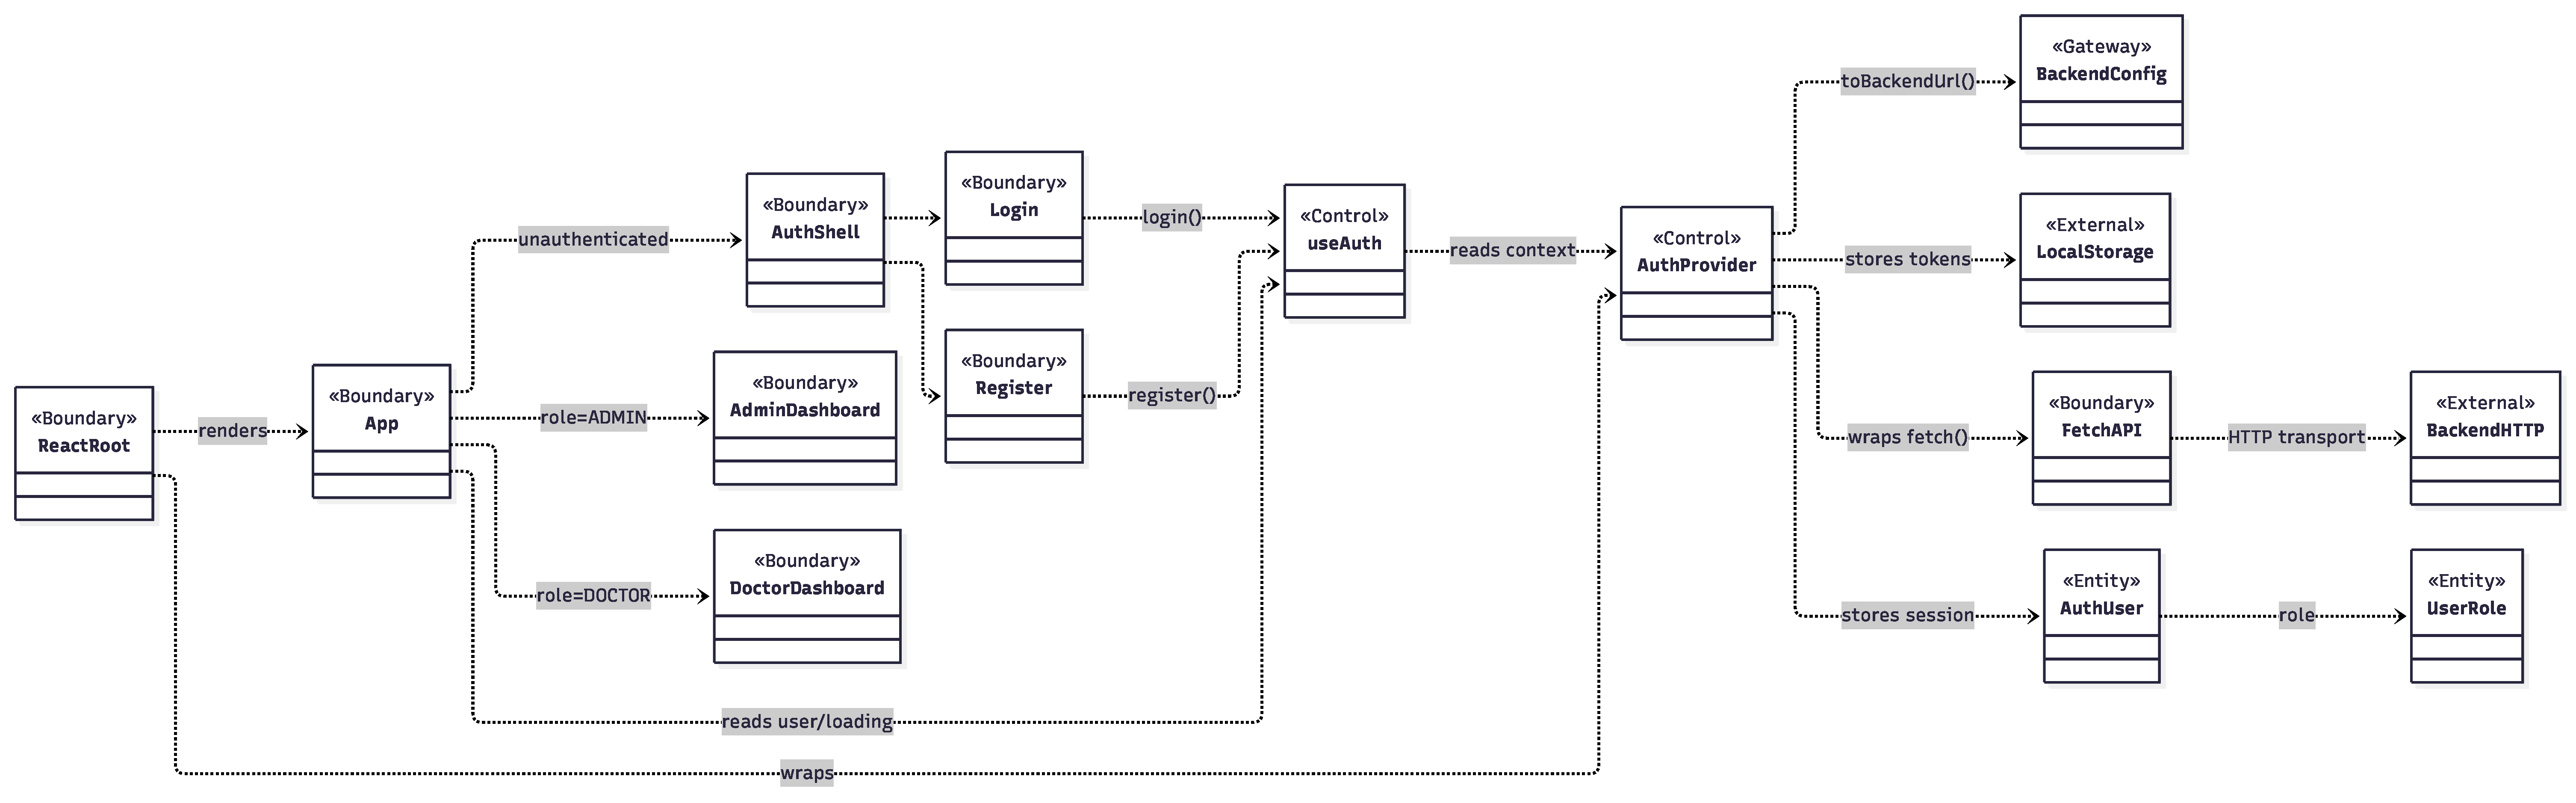
\includegraphics[width=\textwidth]{figures/diagrams/frontend-class-diagram-1.pdf}
    \caption{Bootstrap și autentificare (App Shell).}
    \label{fig:frontend-ecb-auth}
  \end{subfigure}

  \vspace{0.6em}

  \begin{subfigure}[t]{0.7\textwidth}
    \centering
    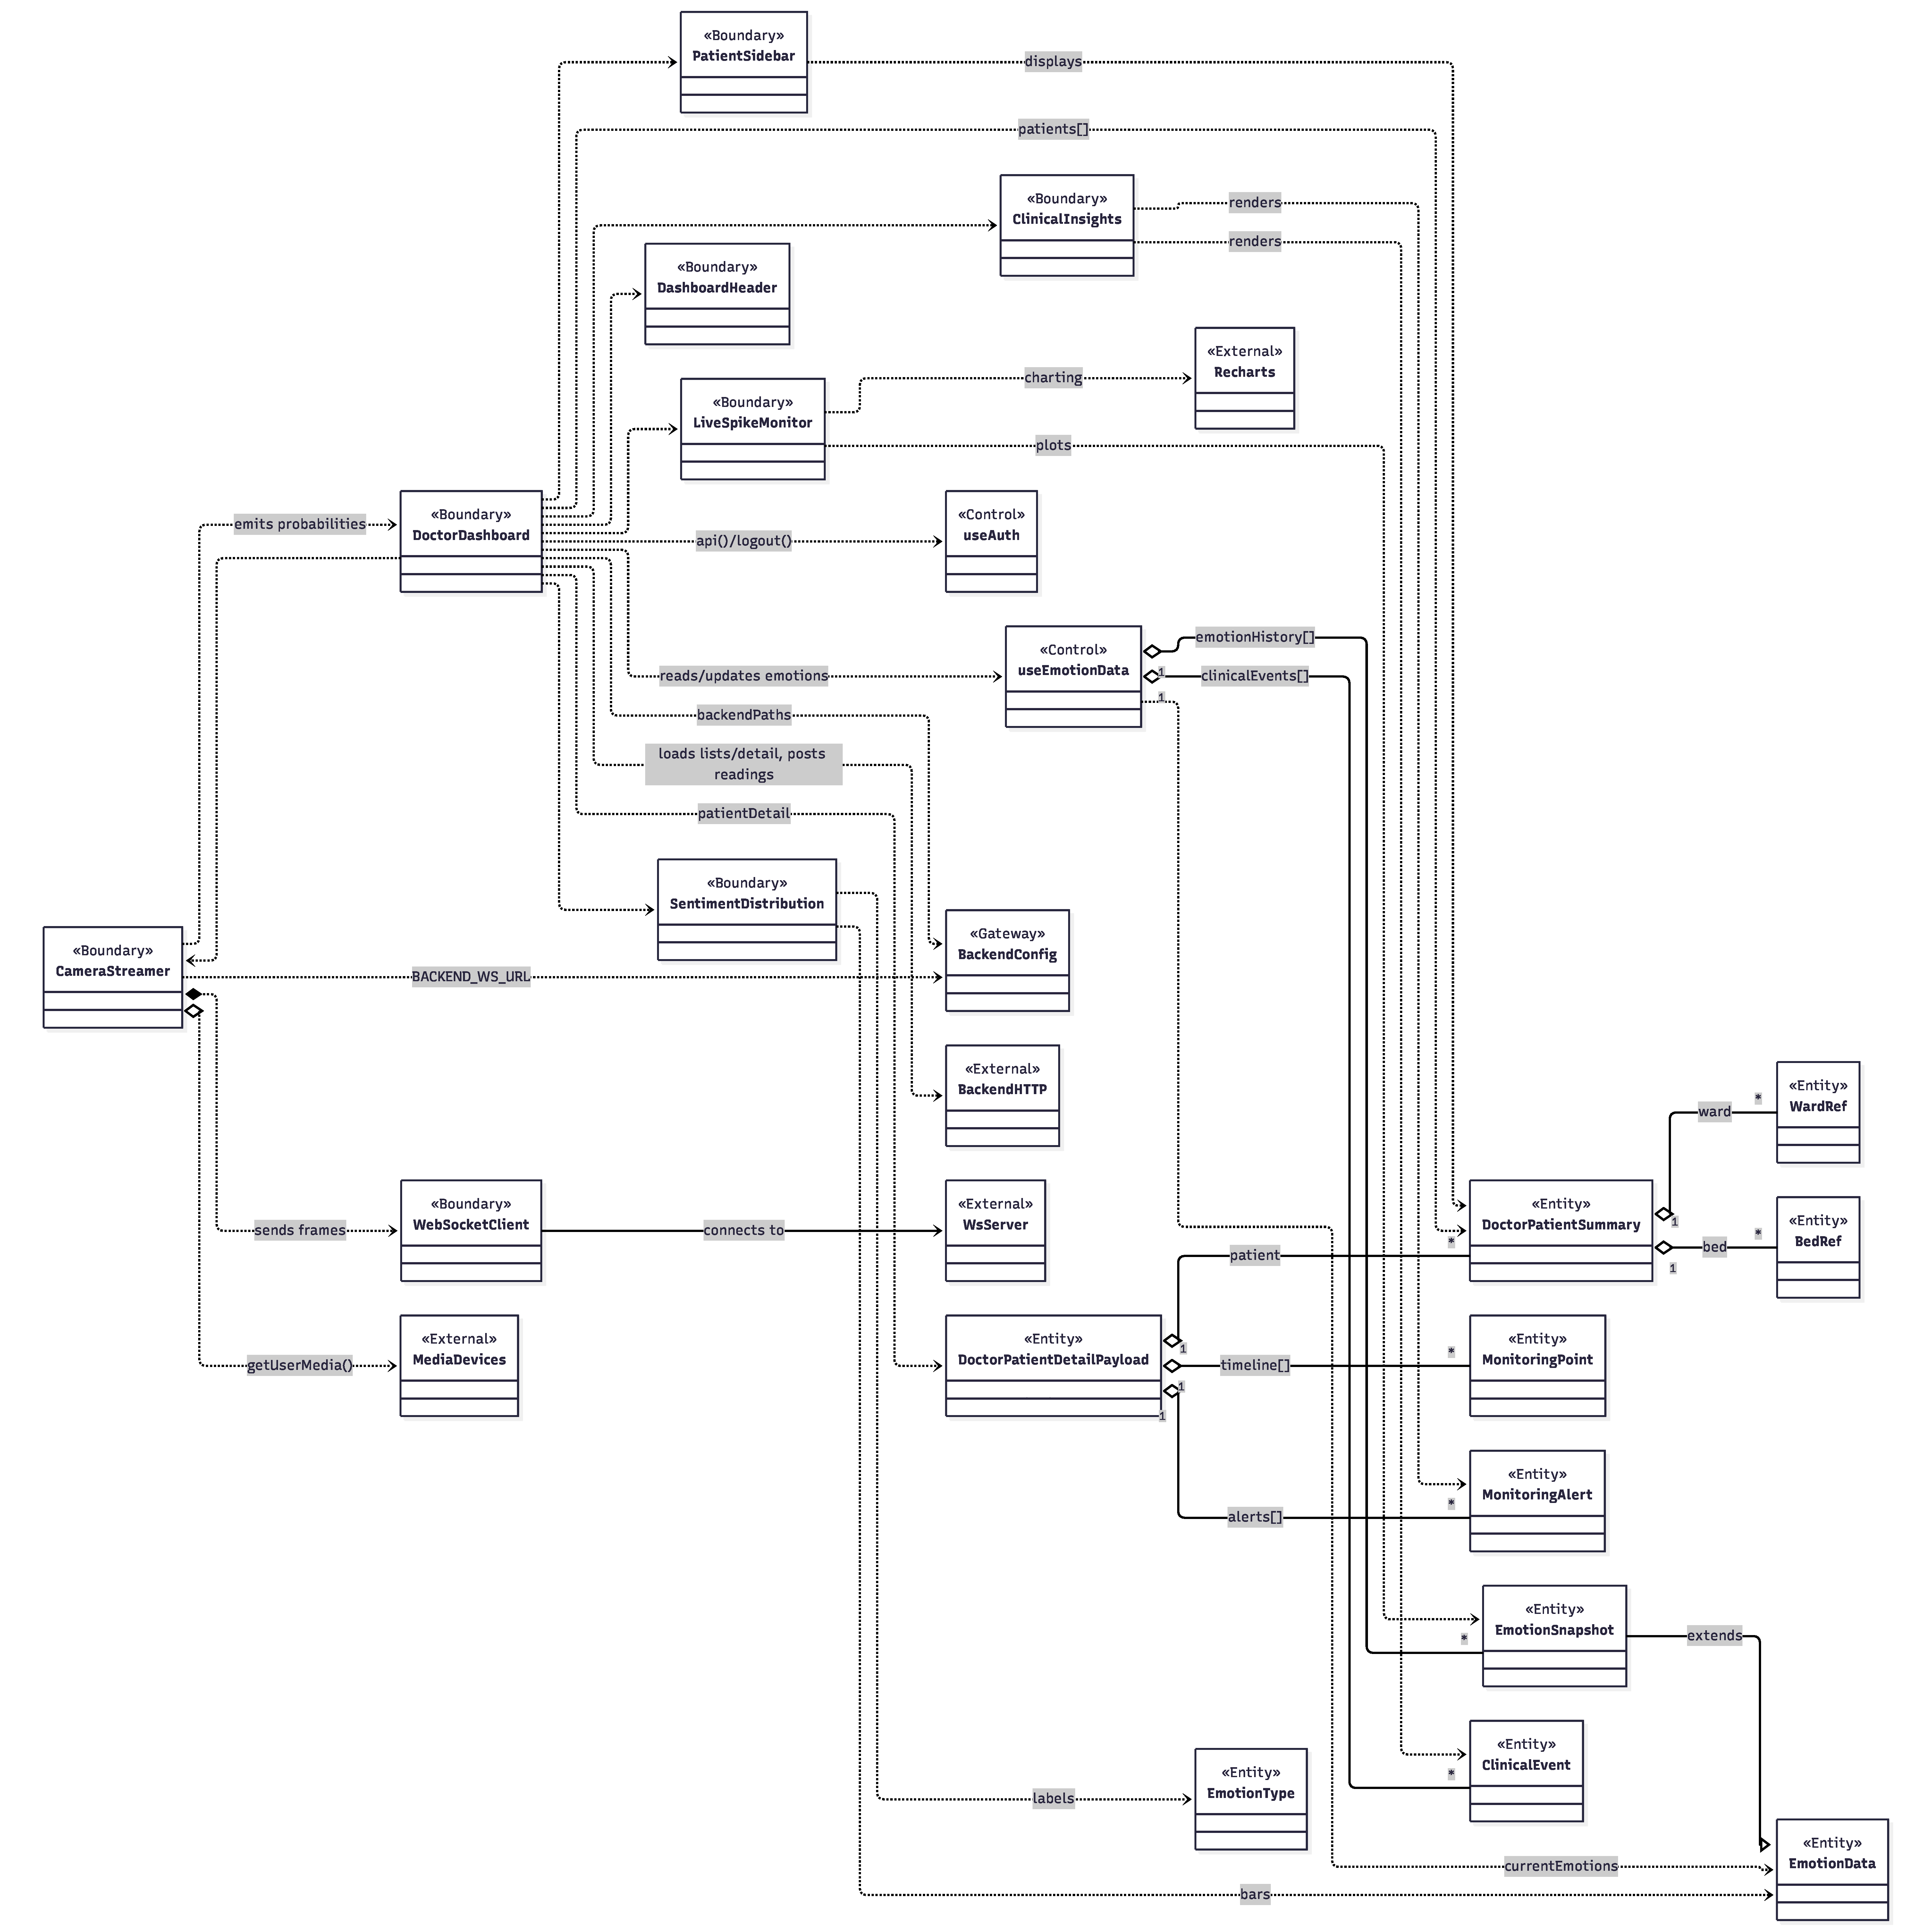
\includegraphics[width=\textwidth]{figures/diagrams/frontend-class-diagram-2.pdf}
    \caption{Fluxul medicului: monitorizare, vizualizare și streaming live.}
    \label{fig:frontend-ecb-doctor}
  \end{subfigure}

  \vspace{0.6em}

  \begin{subfigure}[t]{0.65\textwidth}
    \centering
    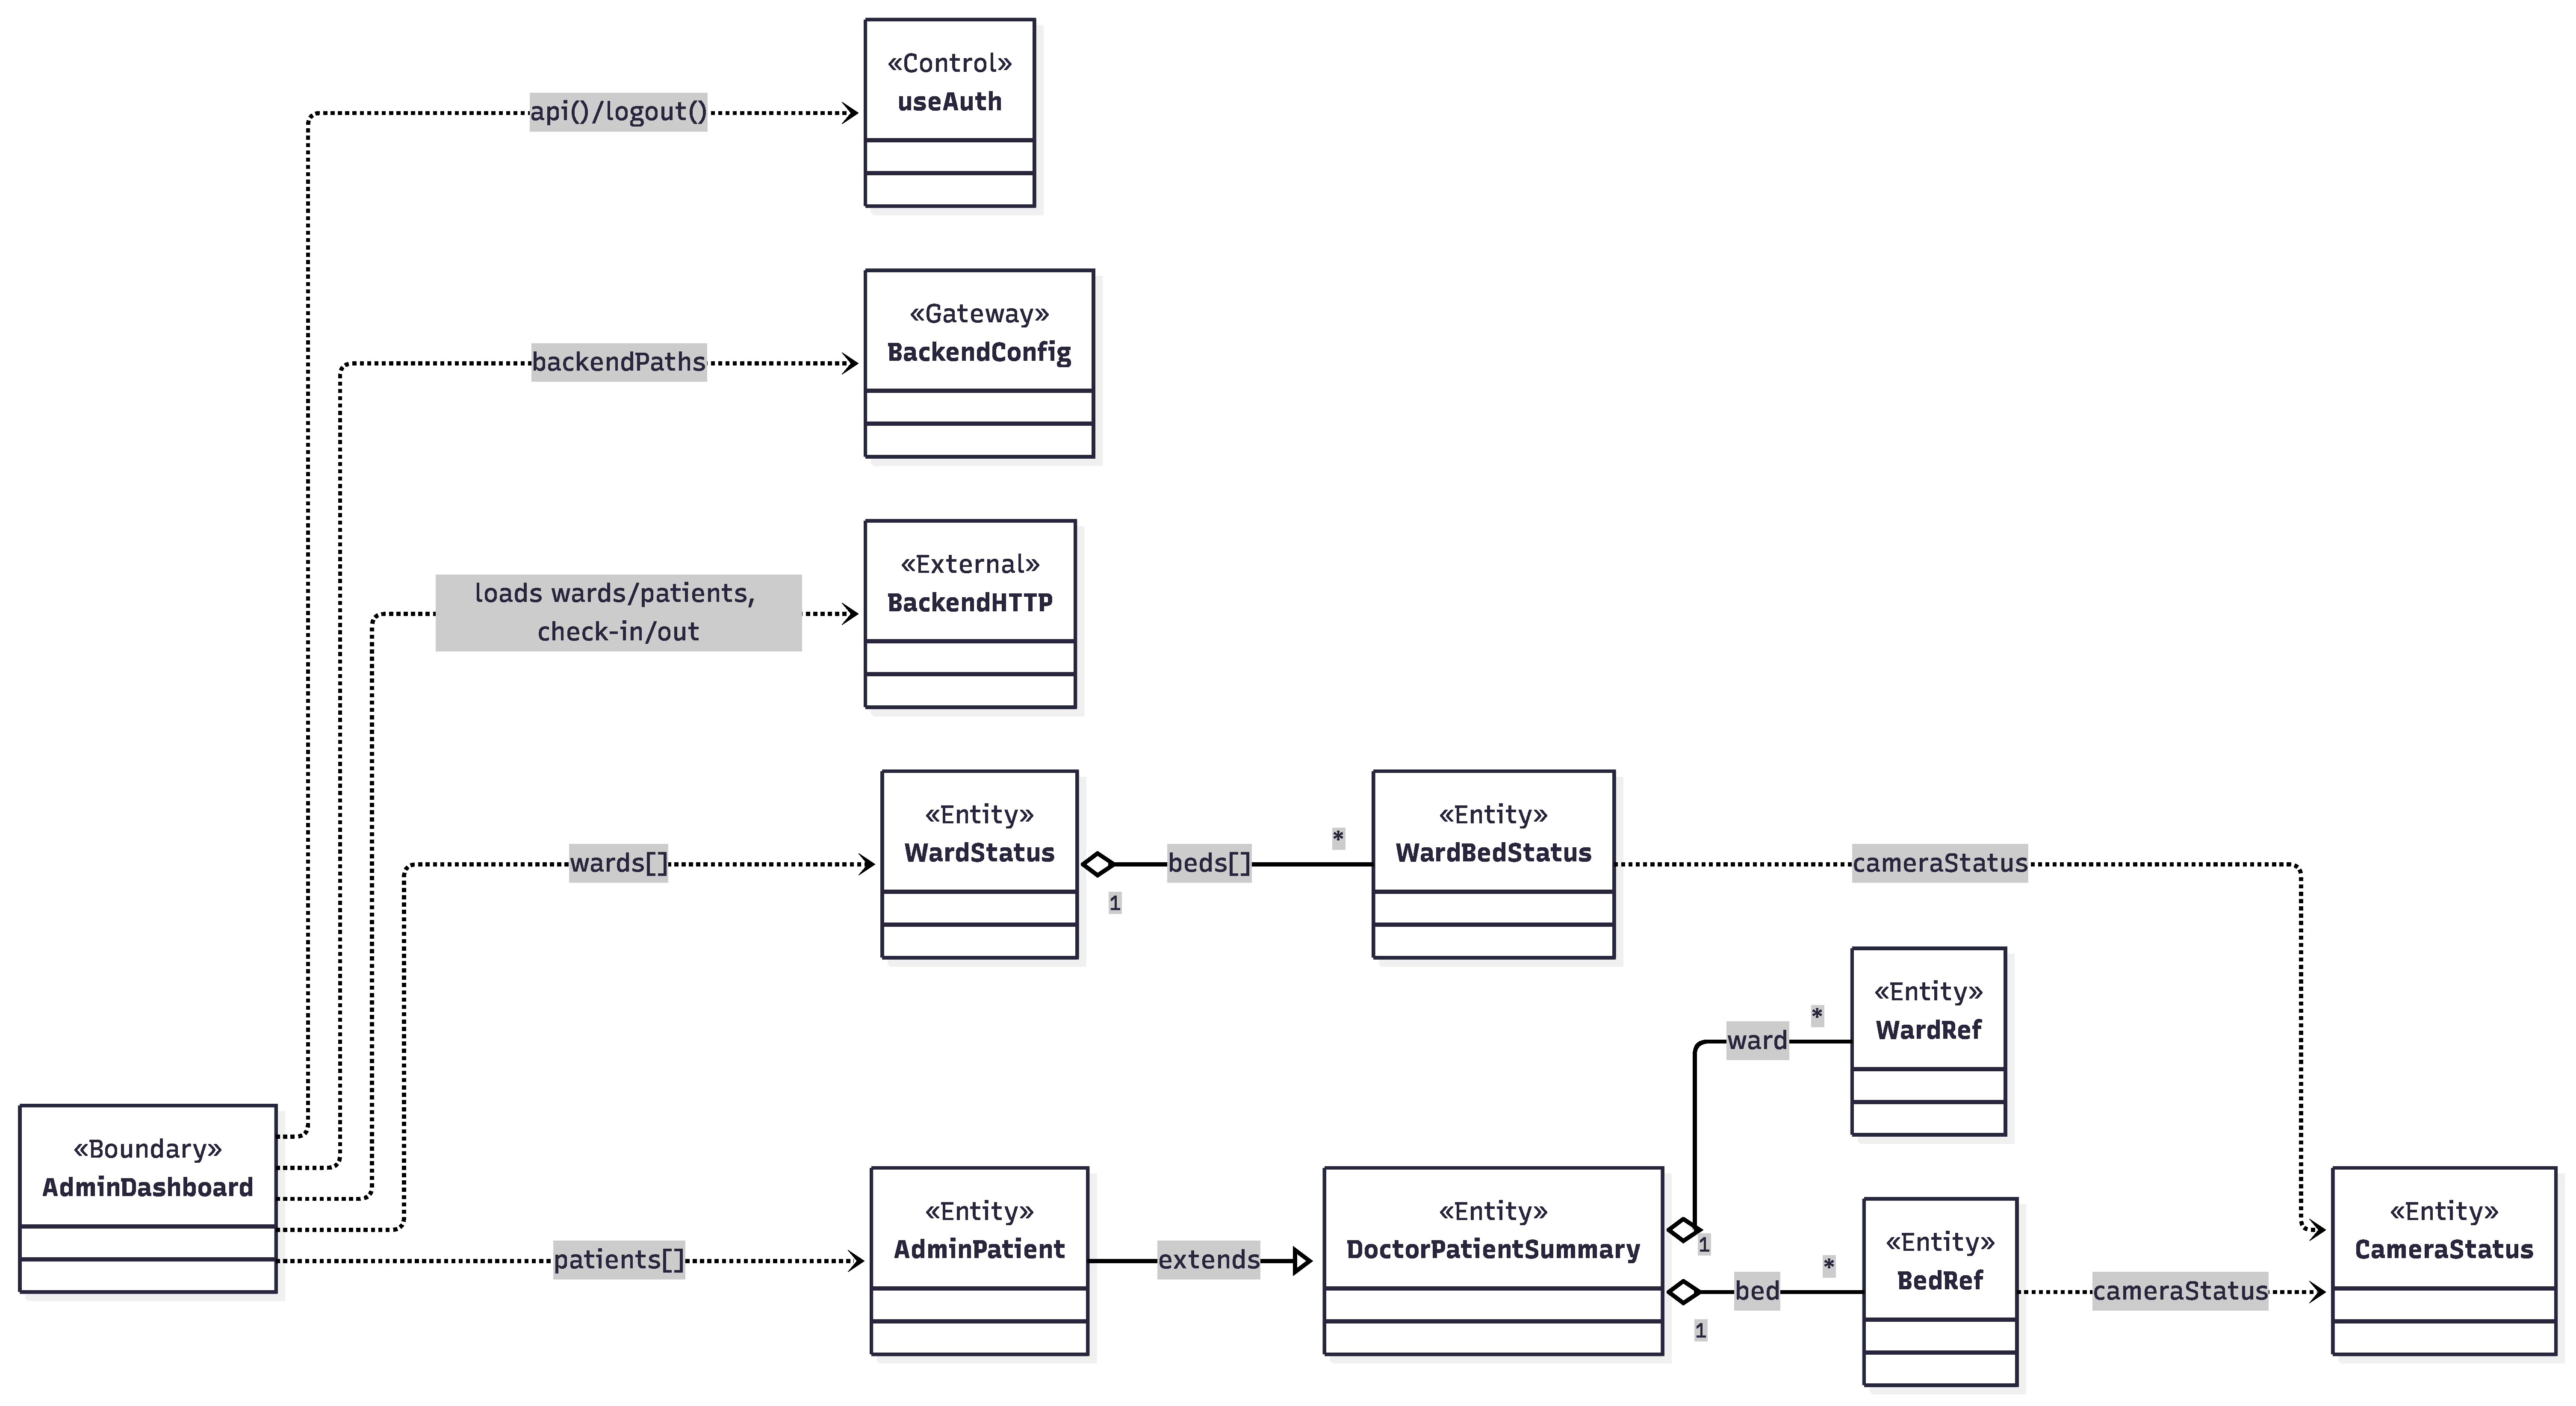
\includegraphics[width=\textwidth]{figures/diagrams/frontend-class-diagram-3.pdf}
    \caption{Fluxul administrativ: management secții/paturi/pacienți.}
    \label{fig:frontend-ecb-admin}
  \end{subfigure}

  \caption{Modelul structural al frontend-ului, conform ECB (Entity--Control--Boundary), extins cu Gateway și External.}
  \label{fig:frontend-ecb}
\end{figure}

Figura~\ref{fig:frontend-ecb} prezintă structura frontend-ului (React + TypeScript) folosind aceeași separare ECB ca în backend, însă cu o nuanță importantă: \textit{Entity} reprezintă în principal \textbf{modele de date/DTO-uri și stări UI} (de ex. \textit{AuthUser}, \textit{DoctorPatientSummary}, \textit{MonitoringPoint}), nu entități persistate direct în aplicația client. \textit{Control} grupează logica de orchestrare (hook-uri precum \textit{useAuth}, \textit{useEmotionData} și provider-ul \textit{AuthProvider}), iar \textit{Boundary} include paginile și componentele UI (de ex. \textit{App}, \textit{DoctorDashboard}, \textit{CameraStreamer}, \textit{LiveSpikeMonitor}). Pentru integrare, sunt evidențiate și componente \textit{Gateway}/\textit{External}, care izolează accesul la resurse de infrastructură (configurația către backend, transport HTTP/WS, API-uri ale browserului).

În Figura~\ref{fig:frontend-ecb-auth} este surprinsă fundația aplicației: \textit{ReactRoot} compune \textit{AuthProvider} peste \textit{App}, iar aplicația decide ruta principală în funcție de sesiune și rol. \textit{AuthProvider} centralizează autentificarea și persistă token-urile în \textit{LocalStorage}, oferind un API unificat pentru cereri HTTP (prin \textit{FetchAPI} și configurarea adreselor prin \textit{BackendConfig}). Această separare reduce duplicarea și menține componentele de UI independente de detaliile de transport.

Figura~\ref{fig:frontend-ecb-doctor} descrie fluxul principal al medicului: \textit{DoctorDashboard} încarcă lista de pacienți și detaliile de monitorizare din backend (DTO-uri precum \textit{DoctorPatientDetailPayload}, \textit{MonitoringPoint}, \textit{MonitoringAlert}), apoi compune componente specializate pentru vizualizare și suport decizional. Starea „live” a sesiunii este gestionată de \textit{useEmotionData} (entități UI precum \textit{EmotionData}, \textit{EmotionSnapshot}, \textit{ClinicalEvent}), în timp ce \textit{CameraStreamer} folosește \textit{MediaDevices} pentru captură și un \textit{WebSocketClient} dedicat pentru trimiterea frame-urilor către backend. Probabilitățile primite sunt propagate către dashboard pentru actualizarea UI și, periodic, pentru persistență prin endpoint-urile HTTP (ex. trimiterea de readings).

În Figura~\ref{fig:frontend-ecb-admin} este reprezentat fluxul administrativ, unde \textit{AdminDashboard} gestionează operațiile de check-in/check-out și statusul secțiilor/paturilor folosind DTO-uri precum \textit{WardStatus}, \textit{WardBedStatus} și \textit{AdminPatient}. Ca și în cazul medicului, comunicarea cu backend-ul este abstractizată prin \textit{useAuth} și aceeași infrastructură de transport/configurare, menținând UI-ul concentrat pe logică de prezentare și pe interacțiunile specifice rolului.

\subsection{Diagrama entitate--relație (ER)}
\label{subsec:model-structural-er}

\begin{figure}[htbp]
  \centering
  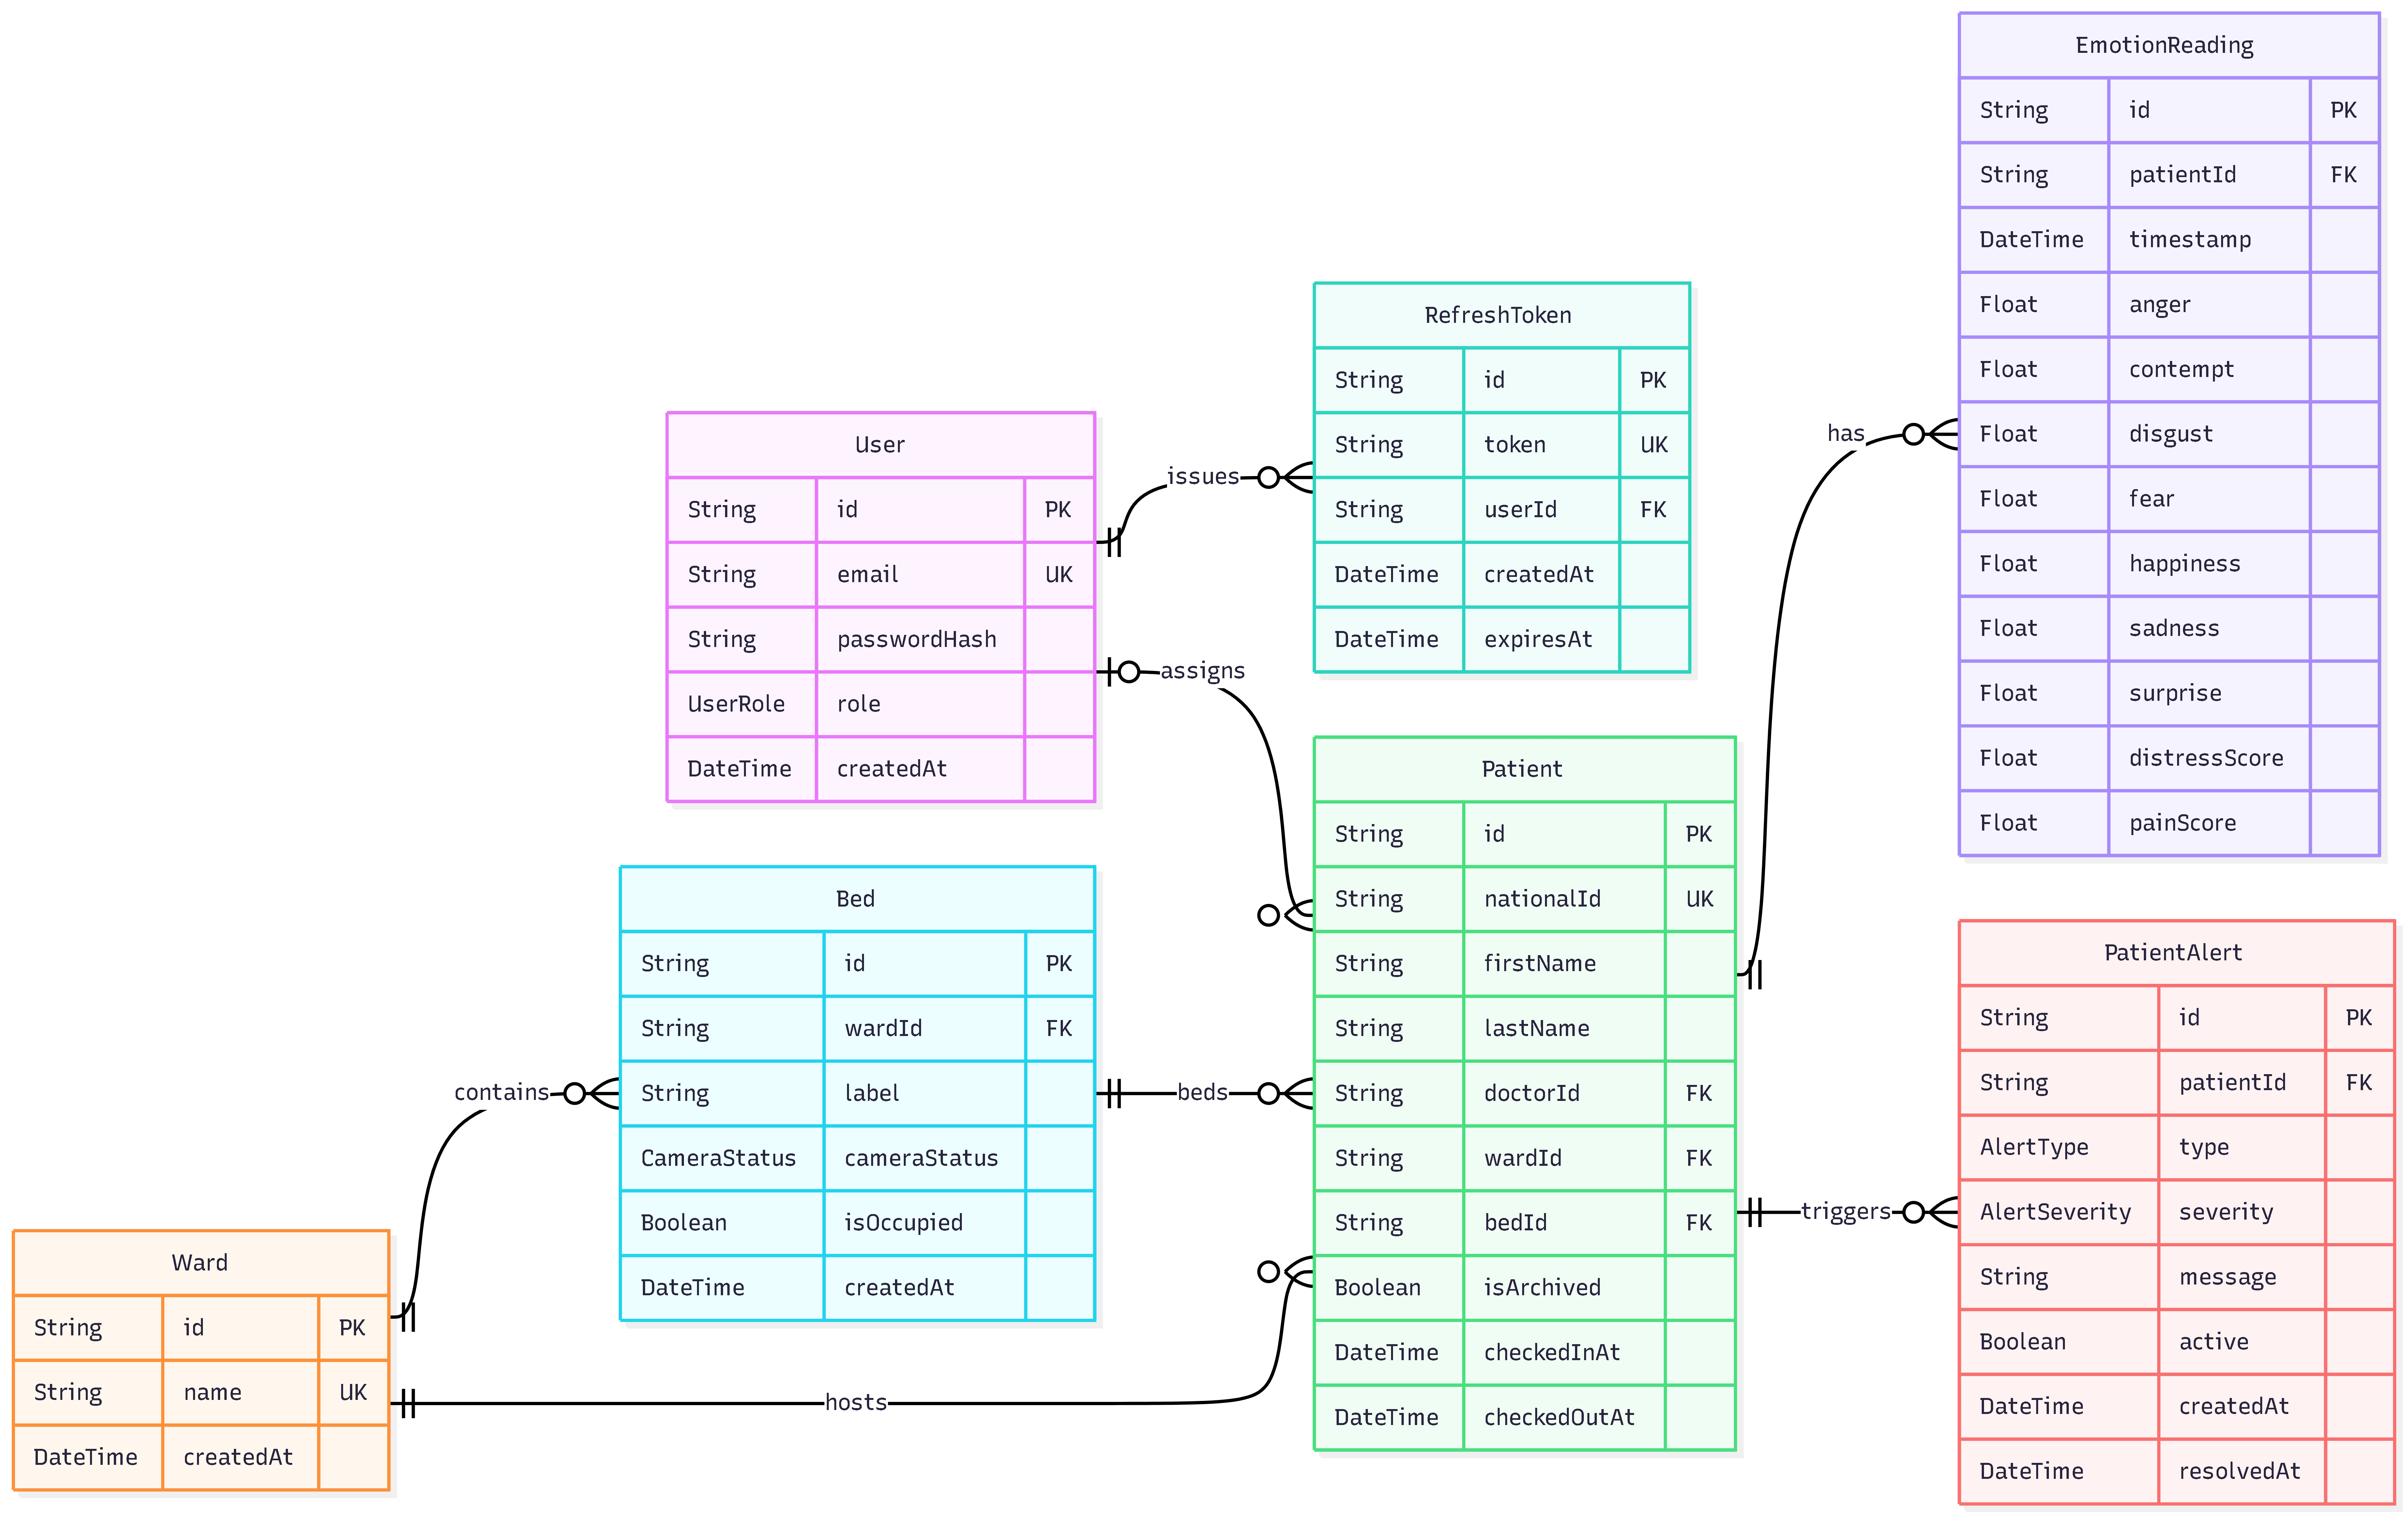
\includegraphics[width=0.9\textwidth]{figures/diagrams/entity_relationship_diagram.png}
  \caption{Diagrama entitate--relație (ER) a bazei de date.}
  \label{fig:backend-er}
\end{figure}

Figura~\ref{fig:backend-er} prezintă modelul relațional al datelor persistente utilizate de aplicație, complementând diagramele ECB. Dacă în modelul structural \textit{Entity} apare ca „nucleu al domeniului”, diagrama ER detaliază modul în care acest nucleu este implementat în baza de date: chei primare, chei străine, constrângeri de unicitate și relațiile dintre entități (cardinalități).

Zona de autentificare este compusă din \textit{User} și \textit{RefreshToken}: fiecare utilizator poate emite mai multe refresh token-uri (relația \textit{User}--\textit{RefreshToken}), iar câmpul \textit{role} (\textit{UserRole}) diferențiază fluxurile și permisiunile din aplicație (medic vs. administrator). La nivel operațional, aceste entități susțin sesiuni persistente și controlul accesului pe roluri.

Modelarea spitalului și a monitorizării este structurată în jurul entității \textit{Patient}, care este asociată cu o secție (\textit{Ward}) și un pat (\textit{Bed}), iar opțional poate fi asignată unui medic (\textit{User}). Starea clinică în timp este capturată prin \textit{EmotionReading} (seturi de valori pe emoții + scoruri agregate), legate de pacient, iar evenimentele de risc sunt reprezentate prin \textit{PatientAlert} (tip, severitate, activ/rezolvat). În acest fel, baza de date relațională păstrează atât structura organizațională (secții/paturi/pacienți), cât și istoricul și semnalările necesare fluxurilor din interfața medicului și a administratorului.

\section{Modelul dinamic al sistemului}
\label{sec:model-dinamic}

\subsection{Diagrama de secvență: Monitorizare live}
\label{subsec:model-dinamic-secventa-live}

\begin{figure}[htbp]
  \centering
  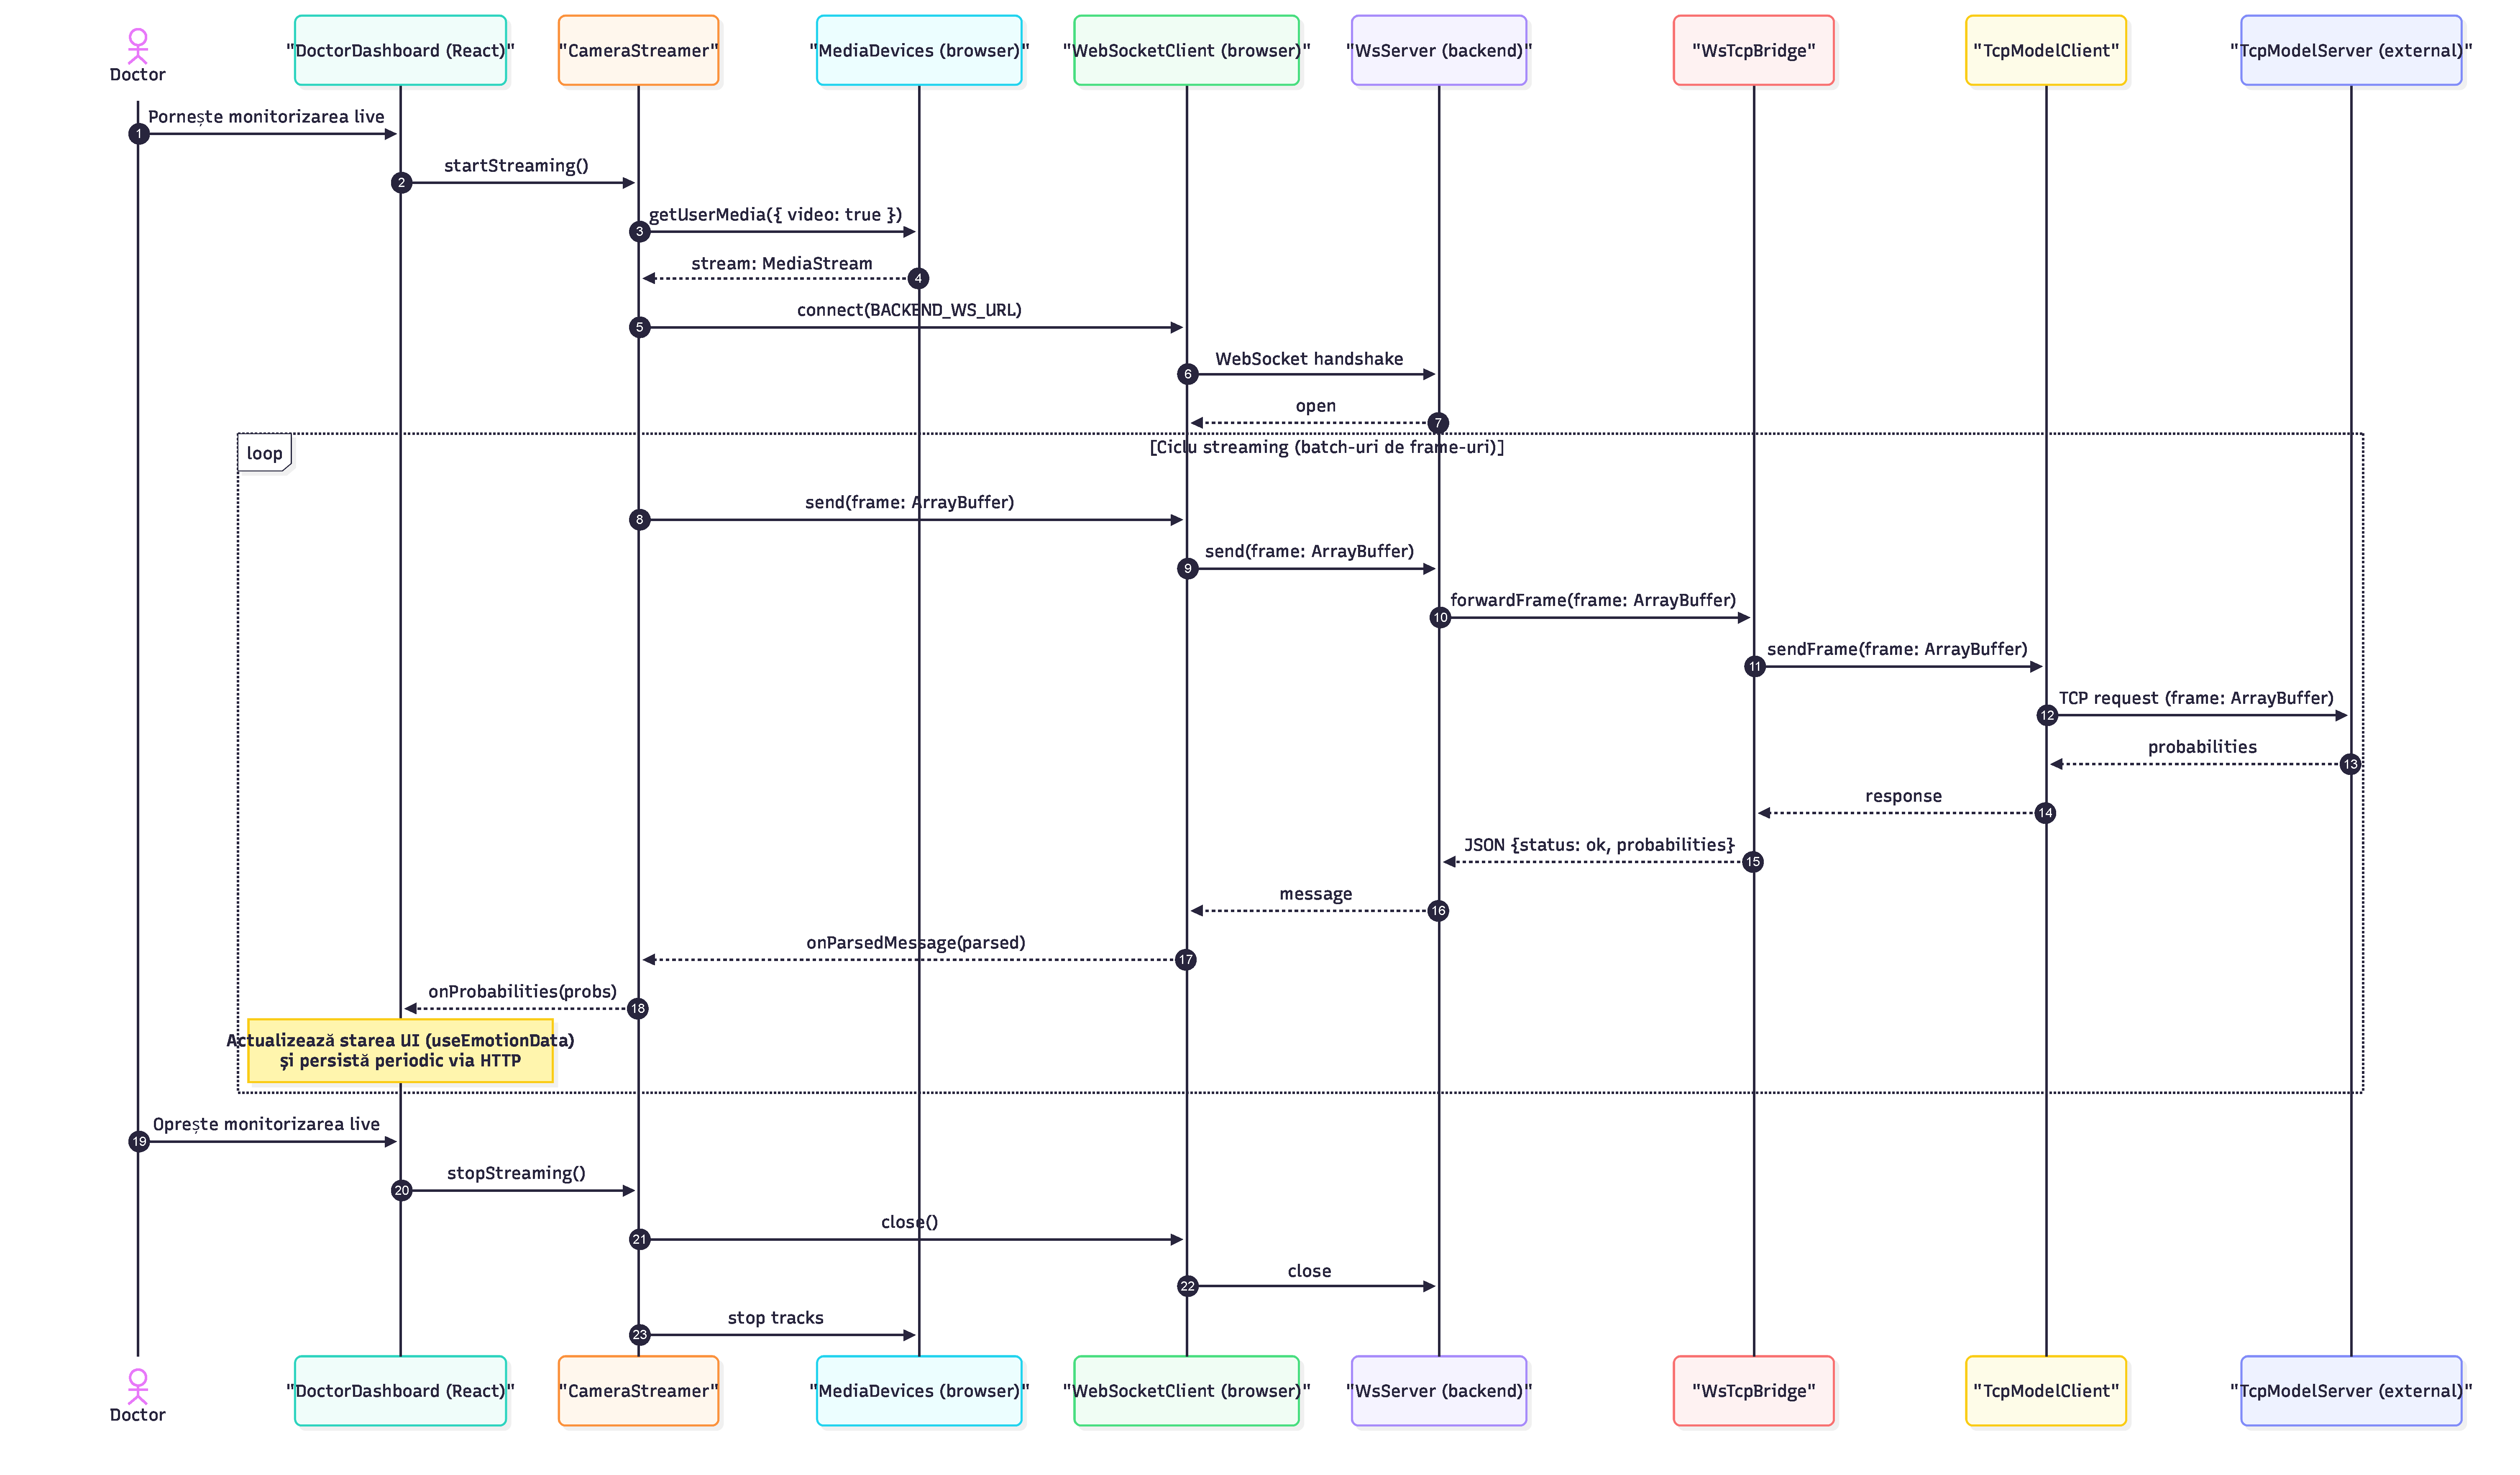
\includegraphics[width=0.99\textwidth]{figures/diagrams/diagrama-SD.pdf}
  \caption{Diagrama de secvență pentru use case-ul \textit{Monitorizare live}: captură video, transmitere prin WebSocket și inferență în model extern (TCP).}
  \label{fig:seq-monitor-live}
\end{figure}

Figura~\ref{fig:seq-monitor-live} descrie fluxul de monitorizare în timp real, declanșat de medic din interfața aplicației. La pornirea sesiunii, componenta de captură inițializează camera folosind API-ul browserului (\textit{MediaDevices}) și stabilește o conexiune WebSocket către backend. Cadrele video sunt pre-procesate (redimensionare/compresie) și transmise ca mesaje binare către server, permițând un canal cu latență redusă față de un flux exclusiv HTTP.

Pe backend, serverul WebSocket primește cadrele și le direcționează către un modul de tip „bridge” care gestionează ordonarea și trimiterea lor către modelul extern. Bridge-ul asigură conectarea către serviciul de inferență (prin clientul TCP) și aplică un mecanism de coadă, astfel încât procesarea să rămână stabilă chiar și când rata de captură depășește temporar capacitatea modelului. Rezultatul inferenței (probabilități pe emoții) este apoi serializat și retransmis prin WebSocket către aplicația web.

La nivel de UI, probabilitățile primite sunt folosite pentru actualizarea stării de monitorizare (grafice, distribuții, evenimente clinice) fără a bloca interacțiunea utilizatorului. Oprirea monitorizării închide conexiunea WebSocket și eliberează resursele de captură (oprirea track-urilor camerei), închizând complet bucla de streaming.

\subsection{Diagrama de comunicare: Vizualizare timeline}
\label{subsec:model-dinamic-comunicare-timeline}

\begin{figure}[htbp]
  \centering
  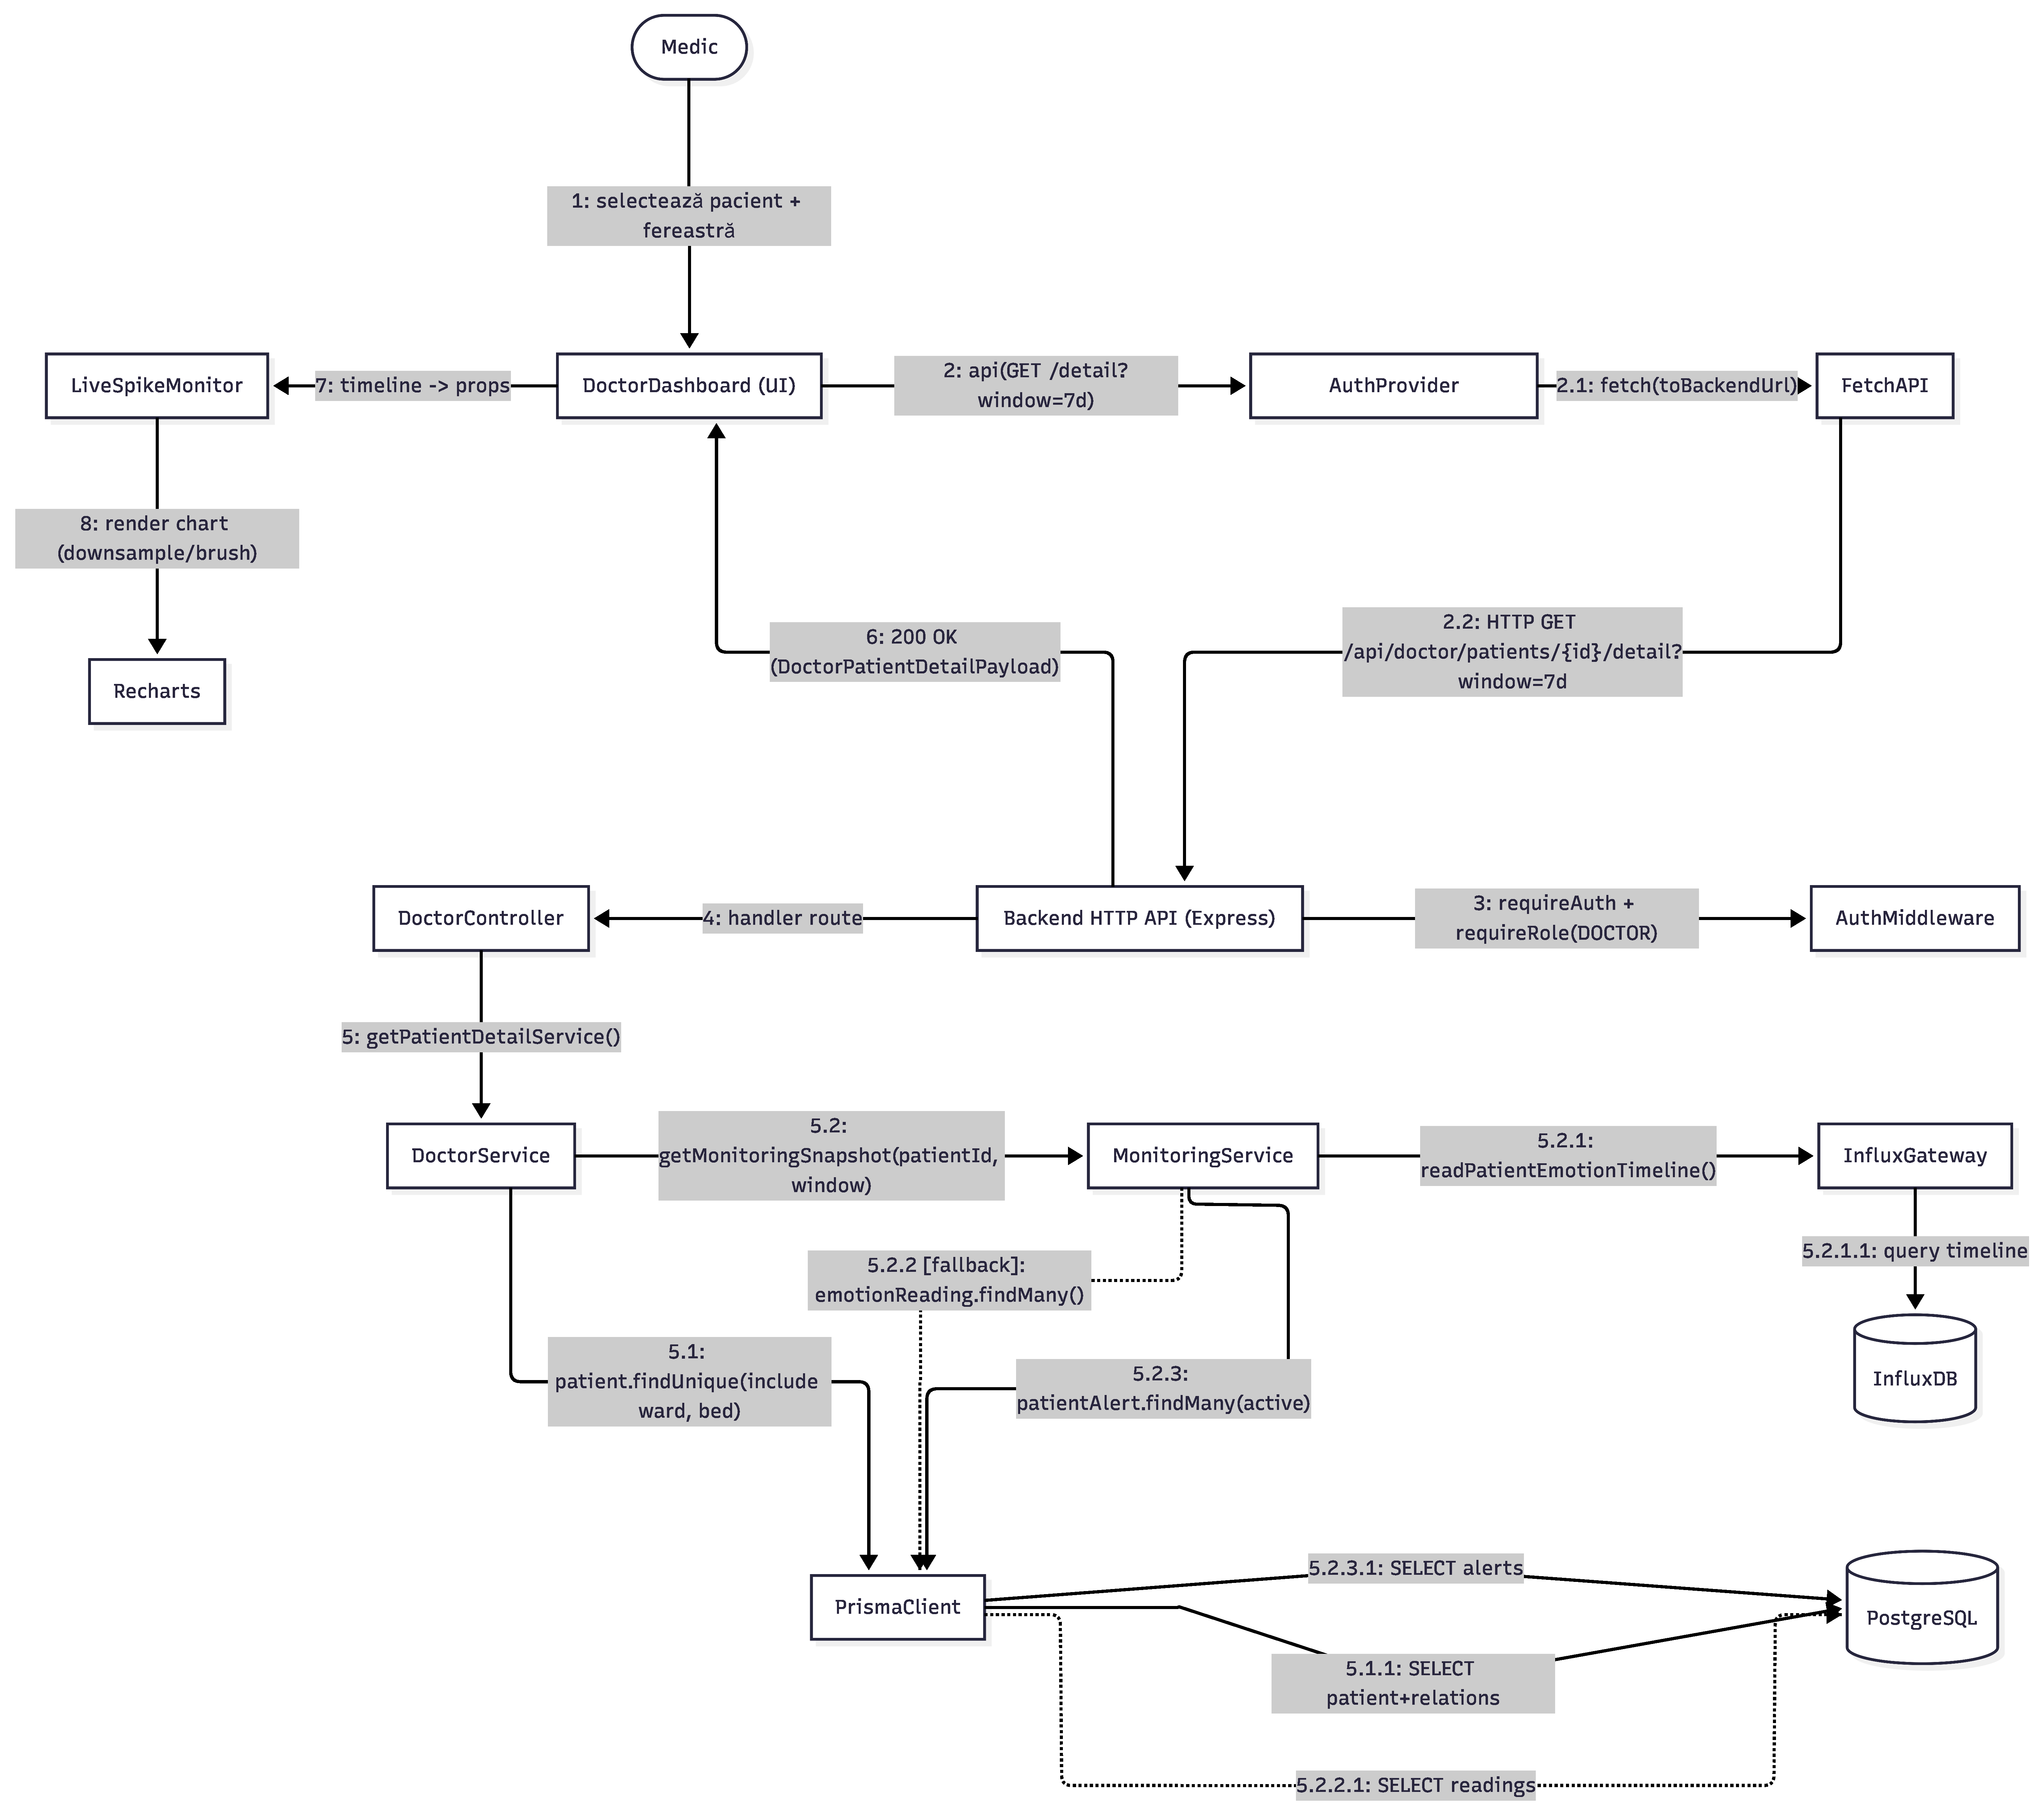
\includegraphics[width=0.7\textwidth]{figures/diagrams/diagrama-CD.pdf}
  \caption{Diagrama de comunicare pentru use case-ul \textit{Vizualizare timeline}.}
  \label{fig:comm-timeline}
\end{figure}

Figura~\ref{fig:comm-timeline} evidențiază participanții și dependențele dintre ei pentru afișarea timeline-ului clinic. Interfața medicului declanșează cererea \texttt{/detail}, autorizată prin token JWT, proces prin care backend-ul orchestrează încărcarea metadatelor pacientului și a istoricului de monitorizare. Datele istorice, denumite \texttt{timelineHistory}, sunt preluate preferențial din \textit{InfluxDB} via \textit{gateway}, aplicându-se un mecanism de \textit{fallback} pe \textit{PostgreSQL} în cazul indisponibilității bazei de date temporale. La fiecare nouă inferență de emoții aceste date istorice sunt actualizate prin adăugarea ultimelor probabilități primite. Pentru a asigura continuitatea vizuală a graficului și o experiență de utilizare fluidă, sistemul implementează un mecanism de eșantionare locală la nivelul interfeței. Astfel, la fiecare $500$ ms, buffer-ul local de memorie, \texttt{emotionHistory} — care reține datele din ultimele $65$ de minute — este actualizat prin adăugarea de noi puncte de date. În intervalele în care nu sunt recepționate cadre noi de la motorul de inferență AI, valorile emoțiilor sunt menținute constante, corespunzând ultimelor probabilități identificate. Matematic, acest comportament este echivalent cu un filtru de menținere de ordin zero (\textit{Zero-Order Hold}), unde valoarea funcției de stare $E(t)$ rămâne invariantă între două momente de detecție succesive $t_n$ și $t_{n+1}$:\begin{equation}E(t) = E(t_n), \quad \text{pentru} \quad t_n \leq t < t_{n+1}\label{eq:zoh_emotions}\end{equation}În final, payload-ul vizualizat de medic reprezintă o concatenare (\textit{mergedMonitorHistory}) a celor două fluxuri: \texttt{timelineHistory} (datele persistate) și \texttt{emotionHistory} (datele curente din memoria volatilă). Acest set de date unificat este mapat către componenta \textit{LiveSpikeMonitor}, care utilizează biblioteca \textit{Recharts} pentru randarea graficului în timp real, oferind o rezoluție de $0.5$ secunde. Un exemplu vizual intuitiv este oferit în Figura~\ref{fig:visual-timeline}. Alertele actualizate sunt folosite de mecanismul de notificări pentru a anunța doctorul schimbări importante legate de starea emoțională a pacientului. 

\begin{figure}[htbp]
  \centering
  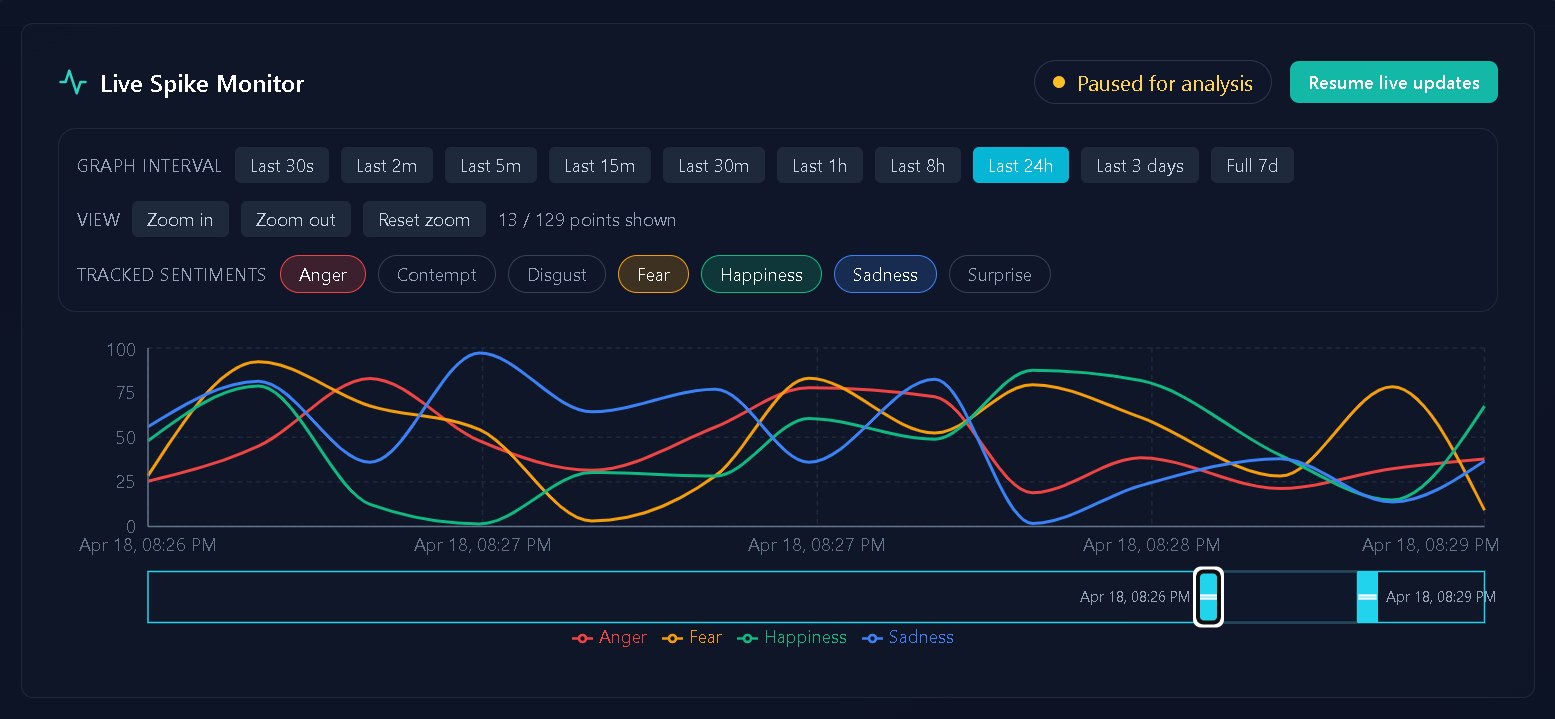
\includegraphics[width=0.99\textwidth]{figures/app/live-spike-monitor.png}
  \caption{Exemplu de vizualizare timeline.}
  \label{fig:visual-timeline}
\end{figure}

\subsection{Diagrama de deployment}
\label{subsec:model-structural-deployment}

\begin{figure}[htbp]
  \centering
  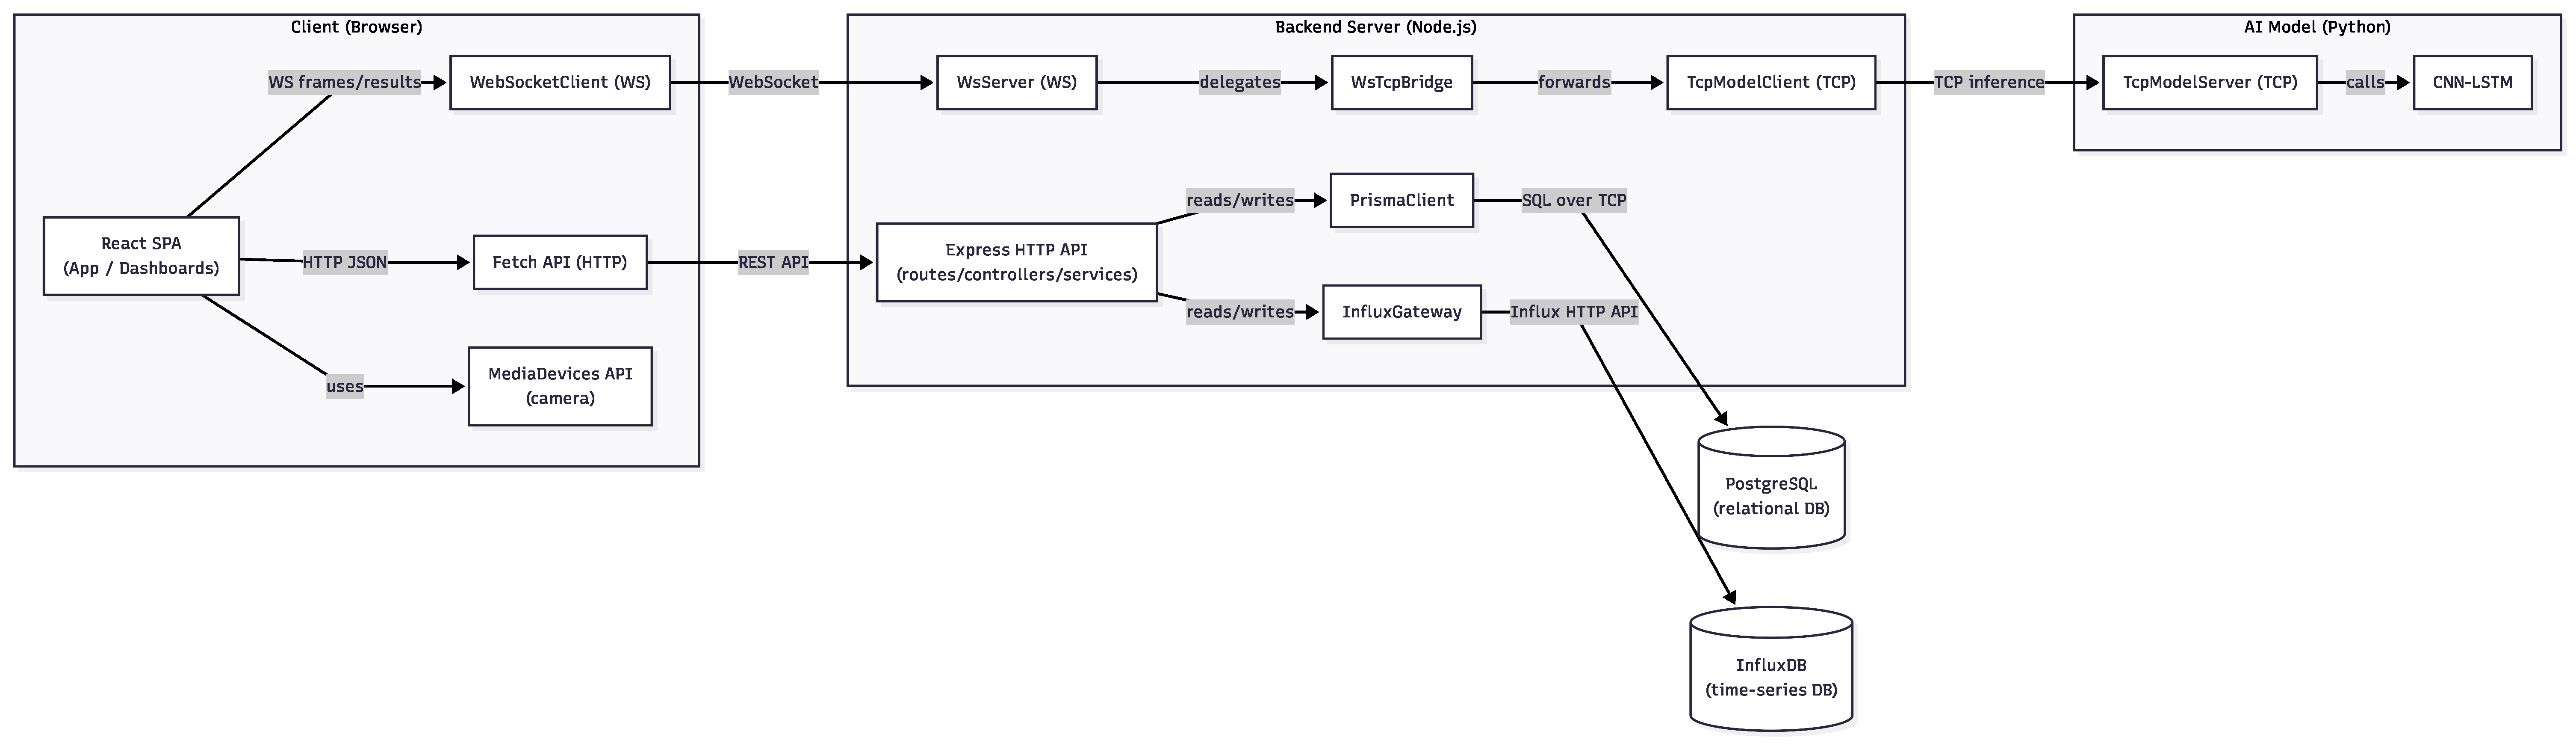
\includegraphics[width=0.99\textwidth]{figures/diagrams/diagrama-deployment.pdf}
  \caption{Diagrama de deployment: noduri de execuție și protocoale de comunicare (REST/HTTP, WebSocket, TCP).}
  \label{fig:deployment}
\end{figure}

Figura~\ref{fig:deployment} evidențiază distribuția fizică a sistemului: aplicația web rulează în browser (interfața React) și comunică cu backend-ul Node.js atât sincron prin REST/HTTP (pentru operații CRUD și încărcarea datelor), cât și asincron prin WebSocket (pentru streaming de cadre și rezultate). Backend-ul accesează persistența relațională în PostgreSQL prin Prisma și utilizează InfluxDB ca depozit time-series pentru timeline-uri, iar inferența este externalizată către un server de model dedicat, accesat prin TCP. Între TCP și WS există o punte de legătură (\textit{TsTcpBridge}) ce asigură comunicarea între cele 2 protocoale.

\subsubsection{Motivația utilizării PostgreSQL + InfluxDB}
\label{subsubsec:postgres-influx-motivatie}

Pentru persistență am ales o abordare hibridă, separând datele \textbf{tranzacționale} (structurate, cu relații) de datele
\textbf{time-series} (flux continuu de puncte indexate temporal). Această separare reduce cuplarea dintre workload-ul de tip OLTP
(operare zilnică, integritate, actualizări) și workload-ul de tip analiză temporală (range queries, agregări pe ferestre).

\begin{itemize}
  \item \textbf{PostgreSQL (bază relațională, sursa de adevăr pentru domeniu clinic).}
  PostgreSQL este utilizat pentru entitățile cu relații clare și reguli de consistență: utilizatori și roluri,
  pacienți, alocarea în salon/pat, stări operaționale, respectiv alertele persistente. Acest tip de date beneficiază direct de:
  \textit{ACID transactions}, constrângeri (chei primare/străine), modelare normalizată, interogări cu \textit{JOIN}-uri și
  migrații controlate ale schemei. Într-un context clinic, aceste proprietăți sunt importante pentru a evita stări invalide
  (ex. pacient fără pat/ward valid sau alerte asociate greșit) și pentru a păstra un istoric coerent.

  \item \textbf{InfluxDB (TSDB pentru timeline-uri și interogări pe intervale de timp).}
  Pentru monitorizarea emoțiilor, aplicația produce un volum mare de puncte cu timestamp (emoții + scoruri derivate),
  interogate aproape exclusiv pe ferestre de timp (ex. ultimele 24h sau 7 zile) și afișate ca grafice.
  O bază de date time-series este optimizată pentru acest tip de acces:
  (i) scrieri frecvente și eficiente, (ii) compresie și stocare eficientă pentru date temporale,
  (iii) interogări rapide de tip \textit{range scan} (``toate punctele dintre $t_0$ și $t_1$''),
  (iv) posibilitatea de a aplica politici de retenție și/sau downsampling fără a afecta modelul relațional.
\end{itemize}

\noindent\textbf{Eficiență și izolare a performanței.}
Deși datele time-series pot fi păstrate și într-o bază relațională, pe măsură ce crește frecvența de eșantionare și retenția,
tabelele mari pot introduce costuri suplimentare (indexuri mai voluminoase, operații de mentenanță, impact asupra latențelor OLTP).
Prin utilizarea InfluxDB pentru timeline-uri, încărcarea asociată interogărilor temporale este mutată către un motor dedicat,
menținând backend-ul și baza relațională responsive pentru operațiile critice (CRUD și tranzacții).

\noindent\textbf{Robustețe operațională (fallback).}
Arhitectura permite ca timeline-ul să fie citit cu prioritate din InfluxDB (dacă este disponibil și are puncte),
iar în caz contrar din persistența relațională; astfel, sistemul rămâne funcțional chiar și în situații de configurare incompletă
sau indisponibilitate temporară a depozitului time-series.

\subsection{Diagrama de stare: \textit{PatientAlert}}
\label{subsec:model-dinamic-stare-patientalert}

\begin{figure}[htbp]
  \centering
  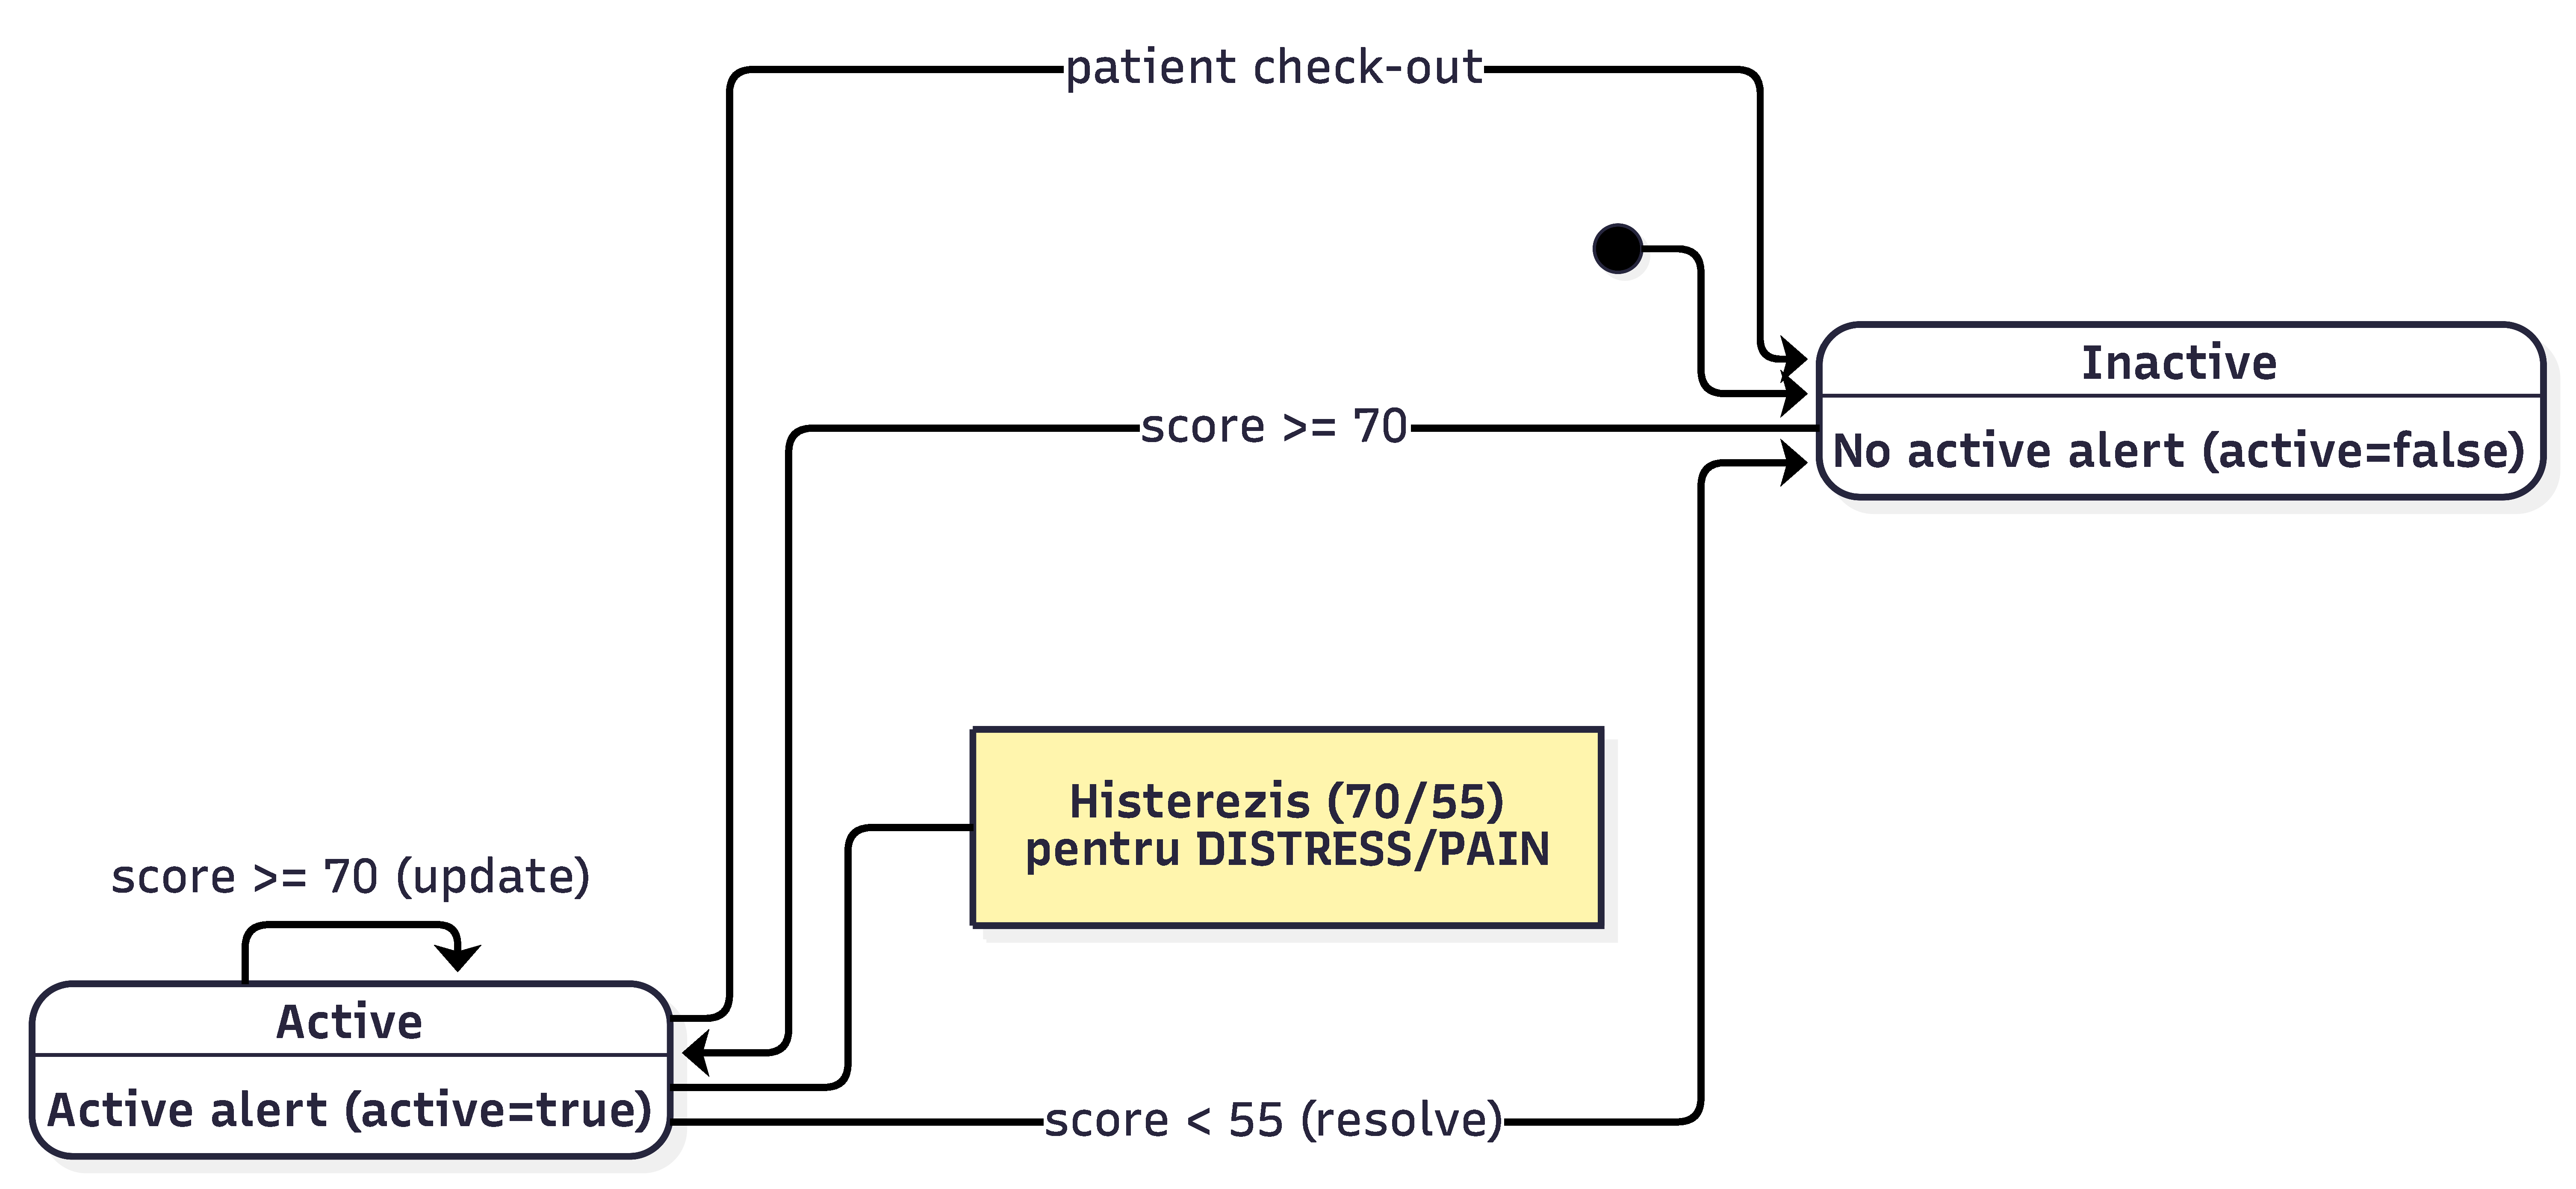
\includegraphics[width=0.6\textwidth]{figures/diagrams/diagrama-stari.pdf}
  \caption{Diagrama de stare pentru \textit{PatientAlert} (per pacient și tip de alertă).}
  \label{fig:state-patientalert}
\end{figure}

Figura~\ref{fig:state-patientalert} descrie ciclul de viață al unei alerte clinice (\textit{DISTRESS}/\textit{PAIN}) asociate unui pacient. Pentru optimizarea mecanismului de declanșare a alertelor și eliminarea fenomenului de instabilitate (\textit{jitter}) la pragurile de decizie, a fost implementat un algoritm de \textbf{histerezis} detaliat în Figura \ref{fig:histerezis_logic}. Acesta utilizează praguri diferențiate pentru activarea ($T_{high} = 70$) și dezactivarea ($T_{low} = 55$) stării de alertă, asigurând astfel o stabilitate temporală a monitorizării și reducând oscilațiile frecvente ale stării.

\begin{figure}[htbp]
    \centering
    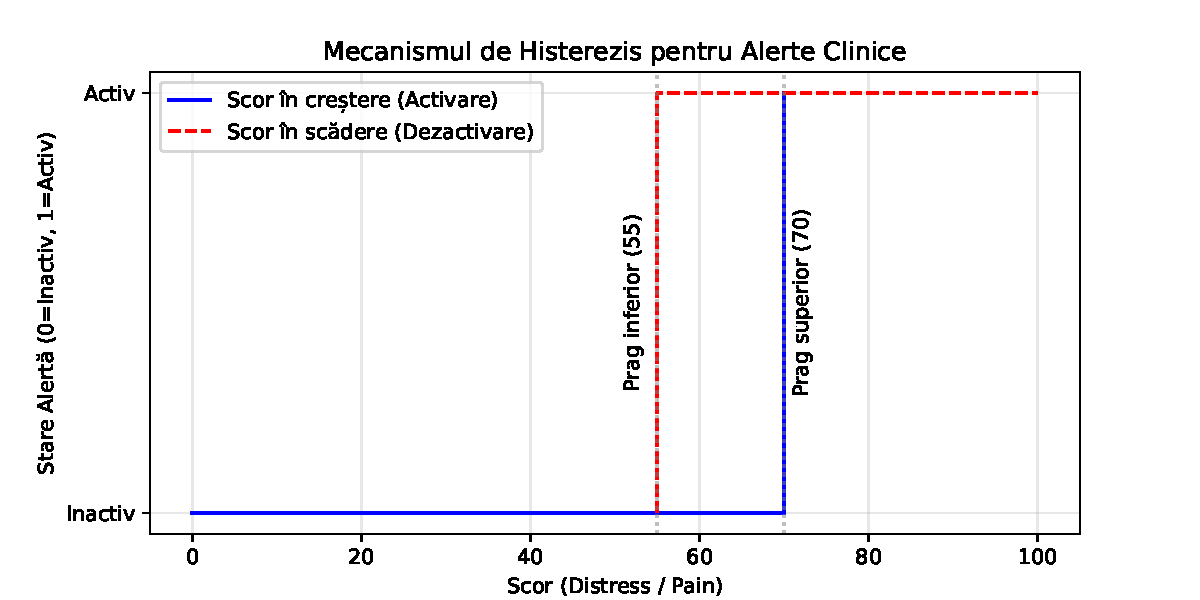
\includegraphics[width=0.8\textwidth]{figures/histerezis_alerte.pdf}
    \caption{Reprezentarea grafică a mecanismului de histerezis aplicat sistemului de alerte. Activarea se produce la depășirea pragului de $70$, în timp ce revenirea la starea inactivă necesită scăderea scorului sub $55$.}
    \label{fig:histerezis_logic}
\end{figure}

Calculul severității se bazează pe două metrici fundamentale, derivate din vectorul stărilor emoționale detectate ($V$). Prima metrică, scorul de \textbf{Distress} ($S_D$), este calculată ca medie aritmetică a stărilor de furie, frică și tristețe, conform ecuației~\eqref{eq:distress_score}:

\begin{equation}
    S_D = \text{clamp}\left(\frac{V_{\text{anger}} + V_{\text{fear}} + V_{\text{sadness}}}{3}, 0, 100\right)
    \label{eq:distress_score}
\end{equation}

Cea de-a doua metrică, scorul de \textbf{Pain} ($S_P$), reprezintă o medie ponderată ce prioritizează frica și tristețea ca indicatori non-verbali ai suferinței fizice, fiind definită în relația~\eqref{eq:pain_score}:

\begin{equation}
    S_P = \text{clamp}\left(0.45 \cdot V_{\text{fear}} + 0.4 \cdot V_{\text{sadness}} + 0.15 \cdot V_{\text{disgust}}, 0, 100\right)
    \label{eq:pain_score}
\end{equation}

În scenariul în care ambele scoruri calculate prin formulele~\eqref{eq:distress_score} și \eqref{eq:pain_score} depășesc pragul critic de activare ($T_{high}$), sistemul aplică o logică de arbitrare prin selecția valorii maxime. Astfel, intensitatea și eticheta alertei sunt determinate de scorul final ($S_{final}$), determinat conform relației~\eqref{eq:final_score}:

\begin{equation}
    S_{final} = \max(S_D, S_P)
    \label{eq:final_score}
\end{equation}

O alertă trece în starea \textit{Active} atunci când valoarea rezultată din ecuația~\eqref{eq:final_score} respectă condiția $S_{final} \geq 70$. În timpul stării active, severitatea și mesajul sunt actualizate dinamic pe baza noilor citiri. Pentru a evita declanșarea repetitivă a notificărilor la fluctuații minore, rezolvarea alertei se produce doar atunci când $S_{final} < 55$, moment în care alertarea este dezactivată și se înregistrează timpul de rezolvare.
Toate aceste actualizări au loc la persistarea unui nou reading de emoții, backendul calculând severitatea pe baza scorului:
  \begin{itemize}
    \item \texttt{HIGH} dacă $\text{score} \ge 85$,
    \item \texttt{MEDIUM} dacă $\text{score} \ge 72$,
    \item \texttt{LOW} în caz contrar.
  \end{itemize}
În interfață, aceste alerte sunt afișate în \textit{Clinical Insights} la secțiunea \textit{Current Alerts} (Figura~\ref{fig:current-alerts}) și reprezintă starea clinică persistată pentru pacient (pe intervalele recente de funcționare).

Sistemul calculează și alerte \textbf{derivate} (nepersistate), pe baza unui \textit{timeline} de emoții pe o fereastră de timp
(ex. 24h sau 7d). Aceste alerte urmăresc episoade susținute, nu doar vârfuri scurte:

\begin{itemize}
  \item Se generează o alertă de tip \texttt{DISTRESS} sau \texttt{PAIN} dacă scorul corespunzător rămâne peste \textbf{65\%}
        timp de cel puțin \textbf{60 minute}.
  \item Mesajul include durata episodului și vârful (peak) atins în acea perioadă.
  \item Severitatea este calculată după aceeași logică (HIGH/MEDIUM/LOW) în funcție de peak.
\end{itemize}

În interfață, aceste alerte apar în \textit{Clinical Insights} la secțiunea \textit{Prolonged Alerts} (Figura~\ref{fig:prolonged-alerts}) și sunt recalculte la fiecare
obținere a unui nou \textit{snapshot} de monitorizare din backend.

\begin{figure}[htbp]
    \centering
    \begin{minipage}{0.48\textwidth}
        \centering
        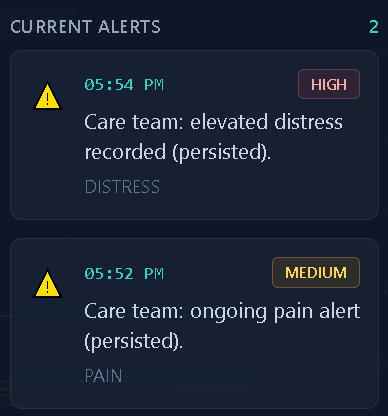
\includegraphics[width=\textwidth]{figures/app/current-alerts.png}
        \caption{Secțiunea \textit{Current Alerts} - vizualizarea alertelor persistente.}
        \label{fig:current-alerts}
    \end{minipage}
    \hfill
    \begin{minipage}{0.48\textwidth}
        \centering
        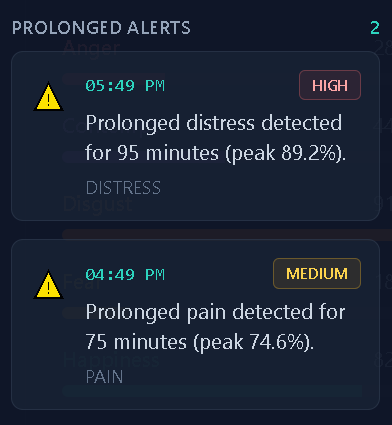
\includegraphics[width=\textwidth]{figures/app/prolonged-alerts.png}
        \caption{Secțiunea \textit{Prolonged Alerts} - vizualizarea alertelor de durată.}
        \label{fig:prolonged-alerts}
    \end{minipage}
\end{figure}

\subsection{Diagrama de activități: Check-in pacient}
\label{subsec:model-dinamic-activity-checkin}

\begin{figure}[htbp]
  \centering
  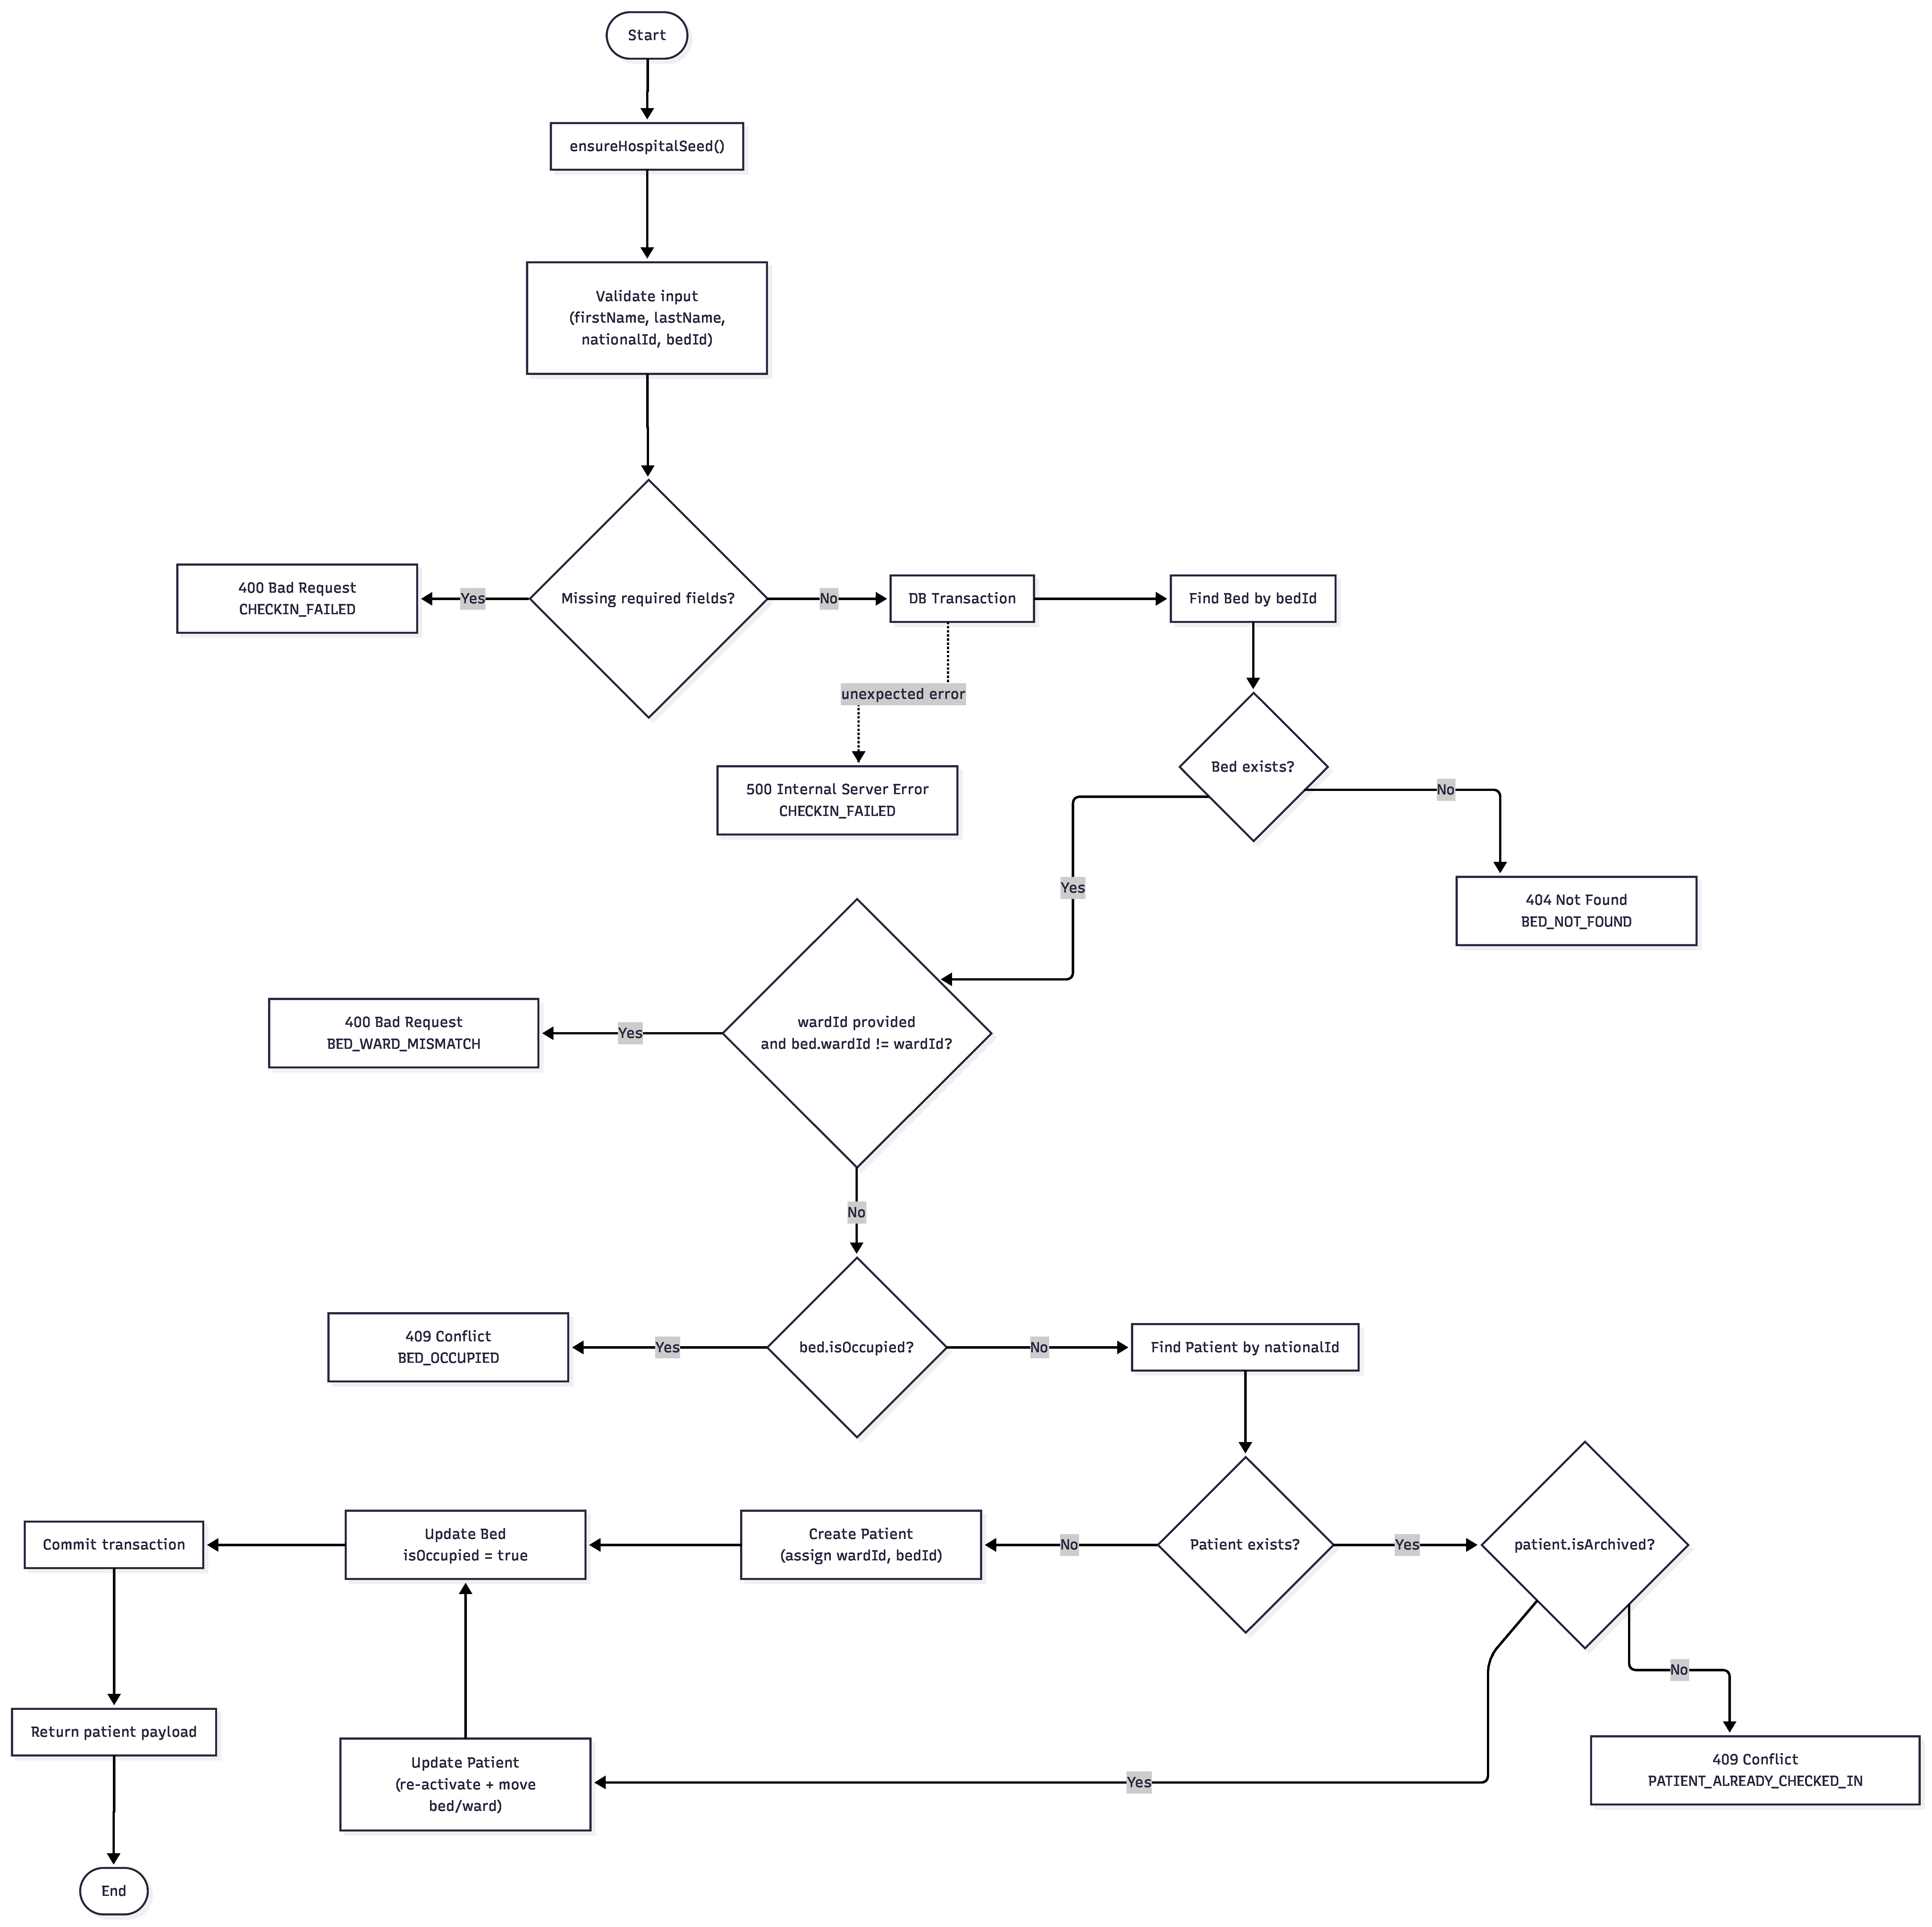
\includegraphics[width=0.97\textwidth]{figures/diagrams/diagrama-activitati.pdf}
  \caption{Diagrama de activități pentru use case-ul \textit{Check-in pacient}.}
  \label{fig:activity-checkin}
\end{figure}

Figura~\ref{fig:activity-checkin} prezintă fluxul operațional de internare (check-in) și deciziile principale care garantează consistența datelor: validarea câmpurilor obligatorii, verificarea existenței patului, compatibilitatea pat--secție (când se indică o secție), și prevenirea ocupării simultane. Operația este tratată tranzacțional, astfel încât înregistrarea/actualizarea pacientului și marcarea patului ca ocupat să fie aplicate atomic. În cazul unui pacient deja internat se returnează un răspuns de tip conflict, iar pentru erori neprevăzute se semnalizează eșecul operației.

\section{Sistemul de alerte și notificări}
\label{sec:sistem-alerte-notificari}

Aplicația integrează un mecanism multi-nivel de alertare, destinat în principal utilizatorului cu rol de medic.
Semnalele sunt generate atât \textbf{în timp real} (din probabilitățile inferate de model), cât și \textbf{la nivel backend}
(din istoricul pacientului și alertele persistate). În plus, există notificări operaționale (erori/stări de funcționare).

\subsection{Evenimente clinice în sesiune (Live Session Events)}
\label{subsec:live-session-events}

La recepționarea fiecărui vector de probabilități de la modelul de inferență, valorile emoționale sunt supuse unui proces de normalizare în intervalul $[0, 100]$, fiind ulterior redate în interfața medicului sub formă de procente. Această vizualizare a emoțiilor curente, exemplificată în Figura~\ref{fig:sentiment-distribution-ui}, oferă o analiză granulară a profilului afectiv, permițând identificarea rapidă a stărilor dominante și a nuanțelor emoționale ale pacientului. Simultan cu afișarea brută a datelor, sistemul execută un mecanism de analiză euristică pentru identificarea episoadelor emoționale semnificative. Se determină emoția dominantă ($E_{max}$) prin identificarea valorii maxime din setul de probabilități curente. Dacă această valoare depășește pragul critic de activare, stabilit la un nivel de încredere de $60\%$, sistemul generează automat un eveniment clinic (\textit{Clinical Event}), conform logicii descrise în relația~\eqref{eq:clinical_event_trigger}:

\begin{equation}
\text{Trigger} = \begin{cases} 
\text{generare eveniment}, & \text{daca} \text{ } \max(V_{\text{emotii}}) > 60 \\ 
\text{stare latenta}, & \text{altfel} 
\end{cases}
\label{eq:clinical_event_trigger}
\end{equation}

Structura și comportamentul acestor evenimente sunt definite prin următoarele caracteristici tehnice, așa cum reiese și din detaliile surprinse în figurile de mai jos:

\begin{itemize}
  \item \textbf{Trigger}: $\max(\text{emotii}) > 60\%$.
  \item \textbf{Conținut}: emoția dominantă, intensitatea (în \%), timestamp și un mesaj selectat aleator din 3 variante predefinite (pentru a evita repetitivitatea).
  \item \textbf{Afișare}: evenimentele apar în panoul \textit{Clinical Insights} la secțiunea \textit{Live Session Events}.
  \item \textbf{Feedback vizual}: emoția detectată este evidențiată temporar (efect de tip \textit{flash/pulse}).
\end{itemize}

\begin{figure}[htbp]
    \centering
    \begin{minipage}{0.35\textwidth}
        \centering
        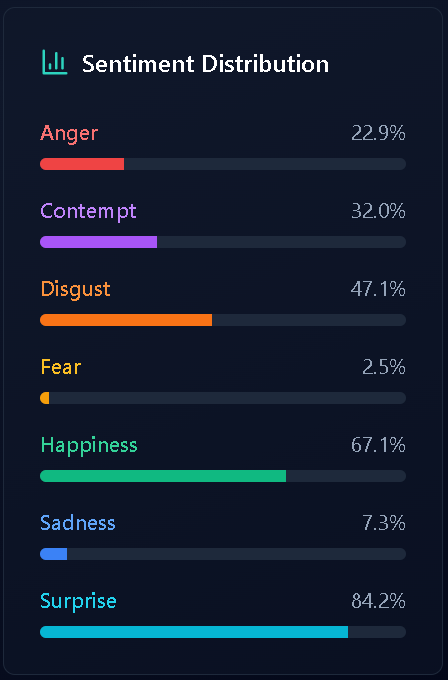
\includegraphics[width=\textwidth]{figures/app/sentiment-distribution.png}
        \caption{Vizualizarea emoțiilor și a intensităților curente.}
        \label{fig:sentiment-distribution-ui}
    \end{minipage}
    \hfill
    \begin{minipage}{0.50\textwidth}
        \centering
        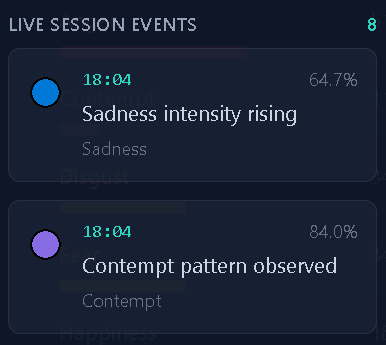
\includegraphics[width=\textwidth]{figures/app/clinical-events.png}
        \caption{Detaliu al panoului \textit{Clinical Insights} cu evenimentele generate.}
        \label{fig:clinical-events-panel}
    \end{minipage}
\end{figure}


\subsection{Indicatori rezumați în UI}
\label{subsec:ui-indicators}

\subsubsection{Clinical Risk Level (Low / Medium / High)}
\label{subsubsec:clinical-risk-level}

În \textit{Patient Sidebar} se afișează nivelul rezumat de risc clinic (\textit{Clinical Risk Level}), derivat din media emoțiilor negative:

\begin{equation}
  \text{avgNegative} = \frac{\text{Anger} + \text{Fear} + \text{Sadness}}{3}
\end{equation}

\begin{equation}
\text{riskLevel} =
\begin{cases}
\text{High}, & \text{dacă } \text{avgNegative} > 50 \\
\text{Medium}, & \text{dacă } \text{avgNegative} > 25 \\
\text{Low}, & \text{altfel}
\end{cases}
\end{equation}

Exemplele vizuale pentru cele trei niveluri sunt prezentate în Figura~\ref{fig:risk-levels}.

\begin{figure}[htbp]
  \centering
  \begin{subfigure}[t]{0.31\textwidth}
    \centering
    
\includegraphics[width=\linewidth]{figures/app/low-clinical-risk-level.png}
    \caption{Low}
    \label{fig:risk-low}
  \end{subfigure}\hfill
  \begin{subfigure}[t]{0.36\textwidth}
    \centering
    
\includegraphics[width=\linewidth]{figures/app/medium-clinical-risk-level.png}
    \caption{Medium}
    \label{fig:risk-medium}
  \end{subfigure}\hfill
  \begin{subfigure}[t]{0.31\textwidth}
    \centering
    
\includegraphics[width=\linewidth]{figures/app/high-clinical-risk-level.png}
    \caption{High}
    \label{fig:risk-high}
  \end{subfigure}
  \caption{Nivelul de risc clinic (Clinical Risk Level) în cele trei stări.}
  \label{fig:risk-levels}
\end{figure}

\subsubsection{Session Type (normal / positive / high-risk)}
\label{subsubsec:session-type}

În header-ul aplicației (lângă titlul platformei) este afișat \textit{Session Type}, care sintetizează rapid starea sesiunii.
Acesta este determinat combinând alertele clinice și emoțiile curente:

\begin{itemize}
  \item \textbf{High-risk}: dacă există cel puțin o alertă cu severitate \texttt{HIGH} (din \textit{Current} sau \textit{Prolonged Alerts})
        \textbf{sau} dacă $\text{Anger} > 60$ și $\text{Fear} > 60$.
  \item \textbf{Positive}: dacă $\text{Happiness} > 50$ și $\text{Surprise} > 30$.
  \item \textbf{Normal}: în celelalte situații.
\end{itemize}

Exemplele vizuale pentru cele trei tipuri sunt prezentate în Figura~\ref{fig:session-types}.

\begin{figure}[htbp]
  \centering
  \begin{subfigure}[t]{0.27\textwidth}
    \centering
    
\includegraphics[width=\linewidth]{figures/app/normal-session.png}
    \caption{Normal}
    \label{fig:session-normal}
  \end{subfigure}\hfill
  \begin{subfigure}[t]{0.32\textwidth}
    \centering
    
\includegraphics[width=\linewidth]{figures/app/positive-engagement-session.png}
    \caption{Positive}
    \label{fig:session-positive}
  \end{subfigure}\hfill
  \begin{subfigure}[t]{0.32\textwidth}
    \centering
    
\includegraphics[width=\linewidth]{figures/app/high-risk-session.png}
    \caption{High-risk}
    \label{fig:session-high-risk}
  \end{subfigure}
  \caption{Tipul sesiunii (\textit{Session Type}) afișat în header, în cele trei stări.}
  \label{fig:session-types}
\end{figure}

\subsection{Notificare la schimbarea nivelului de risc}
\label{subsec:risk-change-notification}

Sistemul urmărește dinamica lui \textit{riskLevel} și notifică medicul \textbf{doar când există o schimbare}:
\begin{itemize}
  \item \textbf{Risk Increased} (degradare): când nivelul trece de la Low $\rightarrow$ Medium/High sau Medium $\rightarrow$ High.
  \item \textbf{Risk Decreased} (îmbunătățire): când nivelul scade (High $\rightarrow$ Medium/Low sau Medium $\rightarrow$ Low).
  \item Dacă nivelul rămâne neschimbat, \textbf{nu se afișează notificare}.
\end{itemize}

Exemplele vizuale ce apar timp de 5 secunde în partea dreaptă de sus pentru cele două situații sunt prezentate în Figura~\ref{fig:risk-notification}.

\begin{figure}[htbp]
  \centering
  \begin{subfigure}[t]{0.30\textwidth}
    \centering
    
\includegraphics[width=\linewidth]{figures/app/risk-increased.png}
    \caption{Notificare de degradare (\textit{Risk Increased}).}
    \label{fig:risk-increased}
  \end{subfigure}\hfill
  \begin{subfigure}[t]{0.34\textwidth}
    \centering
    
\includegraphics[width=\linewidth]{figures/app/risk-decreased.png}
    \caption{Notificare de îmbunătățire (\textit{Risk Decreased}).}
    \label{fig:risk-decreased}
  \end{subfigure}
  \caption{Notificarea afișată la schimbarea nivelului de risc.}
  \label{fig:risk-notification}
\end{figure}

\subsection{Notificări operaționale (erori și stări de funcționare)}
\label{subsec:operational-notifications}

Pe lângă alertarea clinică, aplicația comunică și stări/erori operaționale prin mesaje vizuale:
\begin{itemize}
  \item \textbf{Autentificare}: erori la login/înregistrare (mesaj afișat în formular).
  \item \textbf{Operații de administrare/doctor}: erori la încărcarea listelor sau la acțiuni (ex. preluare pacient, check-in/check-out),
        afișate ca mesaj de eroare în UI.
  \item \textbf{Stare conexiune către model}: indicatori de tip \textit{connected/disconnected}, respectiv stări de captură (\textit{recording/idle}),
        pentru a confirma funcționarea pipeline-ului cameră--model.
\end{itemize}

\section{Testarea aplicației}

\subsection{Rezultatele testarii black-box pentru metoda de inregistrare a citirilor}
\label{subsec:rezultate-blackbox-readings}

Testarea black-box pentru endpoint-ul \texttt{POST /api/doctor/patients/:patientId/readings}
a fost organizata in doua etape: ECP si BVA.
Toate cazurile din suita dedicata au trecut (\textbf{43/43}).

\begingroup
\small
\setlength{\tabcolsep}{6pt}
\renewcommand{\arraystretch}{1.15}

\begin{longtable}{p{1.6cm}p{3.0cm}p{6.8cm}p{2.0cm}p{1.4cm}}
\caption{ECP (Equivalence Class Partitioning) pentru endpoint-ul de readings}
\label{tab:ecp-readings}\\
\toprule
\textbf{ID} & \textbf{Clasa} & \textbf{Date intrare (sinteza)} & \textbf{Rezultat asteptat} & \textbf{Status} \\
\midrule
\endfirsthead

\toprule
\textbf{ID} & \textbf{Clasa} & \textbf{Date intrare (sinteza)} & \textbf{Rezultat asteptat} & \textbf{Status} \\
\midrule
\endhead

\midrule
\multicolumn{5}{r}{\textit{Continua pe pagina urmatoare}} \\
\endfoot

\bottomrule
\endlastfoot

ECP-A1 & Auth invalid & Fara header \texttt{Authorization} & HTTP 401, mesaj \texttt{Missing authorization header} & Pass \\
ECP-A2 & Auth invalid & Header in format gresit (\texttt{Token abc}) & HTTP 401, mesaj \texttt{Invalid authorization format} & Pass \\
ECP-A3 & Auth invalid & JWT invalid (\texttt{Bearer not-a-valid-jwt}) & HTTP 401, mesaj \texttt{Invalid token} & Pass \\
ECP-A4 & Rol nepermis & JWT valid cu rol \texttt{ADMIN} & HTTP 403, mesaj \texttt{Forbidden} & Pass \\

ECP-B1 & Pacient invalid & Pacient inexistent & HTTP 404, mesaj \texttt{Patient not found} & Pass \\
ECP-B2 & Pacient invalid & Pacient arhivat & HTTP 404, mesaj \texttt{Patient not found} & Pass \\
ECP-B3 & Acces nepermis & Pacient alocat altui doctor & HTTP 403, mesaj \texttt{You can only push readings...} & Pass \\

ECP-C1 & Payload valid & Emotii in campul \texttt{probabilities}: Anger/Fear/Sadness & HTTP 201, persistare corecta (normalizare) & Pass \\
ECP-C2 & Payload valid & Emotii in body top-level (\texttt{anger}, \texttt{fear}, \texttt{sadness}) & HTTP 201, persistare corecta & Pass \\
ECP-C3 & Payload invalid & Doar chei nerecunoscute (ex. Joy, Calmness) & HTTP 400, mesaj \texttt{Reading payload does not contain emotion values} & Pass \\
ECP-C4 & Payload invalid & Chei valide, dar valori non-numerice (\texttt{Anger='abc'}) & HTTP 400, mesaj \texttt{Reading payload does not contain emotion values} & Pass \\

ECP-D1 & Timestamp invalid & \texttt{timestamp='invalid-date'} & HTTP 400, mesaj \texttt{Invalid timestamp} & Pass \\
ECP-D2 & Timestamp valid implicit & \texttt{timestamp} lipsa & HTTP 201, timestamp server-side valid & Pass \\

ECP-E1 & Domeniu numeric extins & Valori sub 0 si peste 100 (ex. -10, 150) & HTTP 201, clamp in intervalul [0,100] & Pass \\

ECP-F1 & Alertare - clasa joasa & Distress si pain sub pragul de alertare & HTTP 201, fara creare alerta & Pass \\
ECP-F2 & Alertare - distress dominant & Scoruri ridicate cu distress dominant & HTTP 201, creare alerta \texttt{DISTRESS} (severitate corecta) & Pass \\
ECP-F3 & Alertare - pain dominant & Scoruri ridicate cu pain dominant & HTTP 201, creare alerta \texttt{PAIN} (severitate corecta) & Pass \\
ECP-F4 & Alerta existenta & Exista alerta activa de acelasi tip & HTTP 201, \texttt{update} alerta (nu \texttt{create}) & Pass \\
ECP-F5 & Rezolvare alerta & Scoruri coborate sub prag de rezolvare & HTTP 201, \texttt{resolve} pentru alertele active relevante & Pass \\

\end{longtable}
\endgroup


\begingroup
\small
\setlength{\tabcolsep}{6pt}
\renewcommand{\arraystretch}{1.15}

\begin{longtable}{p{1.6cm}p{3.3cm}p{6.5cm}p{2.0cm}p{1.4cm}}
\caption{BVA (Boundary Value Analysis) pentru endpoint-ul de readings}
\label{tab:bva-readings}\\
\toprule
\textbf{ID} & \textbf{Frontiera} & \textbf{Valoare testata} & \textbf{Rezultat asteptat} & \textbf{Status} \\
\midrule
\endfirsthead

\toprule
\textbf{ID} & \textbf{Frontiera} & \textbf{Valoare testata} & \textbf{Rezultat asteptat} & \textbf{Status} \\
\midrule
\endhead

\midrule
\multicolumn{5}{r}{\textit{Continua pe pagina urmatoare}} \\
\endfoot

\bottomrule
\endlastfoot

BVA-1a & hasData in jurul lui 0 & Anger = -1 & HTTP 400 (fara date emotionale valide) & Pass \\
BVA-1b & hasData in jurul lui 0 & Anger = 0 & HTTP 400 (fara date emotionale valide) & Pass \\
BVA-1c & hasData in jurul lui 0 & Anger = +1 & HTTP 201 (date valide) & Pass \\

BVA-2a & Scalare la pragul 1 & Anger = 0.99 & HTTP 201, normalizare la 99 & Pass \\
BVA-2b & Scalare la pragul 1 & Anger = 1.00 & HTTP 201, normalizare la 100 & Pass \\
BVA-2c & Scalare la pragul 1 & Anger = 1.01 & HTTP 201, valoare ramane 1.01 (fara scalare x100) & Pass \\

BVA-3a & Clamp superior la 100 & Anger = 99 & HTTP 201, valoare 99 & Pass \\
BVA-3b & Clamp superior la 100 & Anger = 100 & HTTP 201, valoare 100 & Pass \\
BVA-3c & Clamp superior la 100 & Anger = 101 & HTTP 201, clamp la 100 & Pass \\

BVA-4a & Prag alertare 70 (\(\pm 1\)) & Distress = 69 & HTTP 201, fara alerta noua & Pass \\
BVA-4b & Prag alertare 70 (\(\pm 1\)) & Distress = 70 & HTTP 201, creare alerta (LOW) & Pass \\
BVA-4c & Prag alertare 70 (\(\pm 1\)) & Distress = 71 & HTTP 201, creare alerta (LOW) & Pass \\

BVA-5a & Prag severitate 72 (\(\pm 1\)) & Scor = 71 & Severitate LOW & Pass \\
BVA-5b & Prag severitate 72 (\(\pm 1\)) & Scor = 72 & Severitate MEDIUM & Pass \\
BVA-5c & Prag severitate 72 (\(\pm 1\)) & Scor = 73 & Severitate MEDIUM & Pass \\

BVA-6a & Prag severitate 85 (\(\pm 1\)) & Scor = 84 & Severitate MEDIUM & Pass \\
BVA-6b & Prag severitate 85 (\(\pm 1\)) & Scor = 85 & Severitate HIGH & Pass \\
BVA-6c & Prag severitate 85 (\(\pm 1\)) & Scor = 86 & Severitate HIGH & Pass \\

BVA-7a & Prag resolve distress 55 (\(\pm 1\)) & Distress = 54 & HTTP 201, se executa resolve DISTRESS & Pass \\
BVA-7b & Prag resolve distress 55 (\(\pm 1\)) & Distress = 55 & HTTP 201, fara resolve DISTRESS & Pass \\
BVA-7c & Prag resolve distress 55 (\(\pm 1\)) & Distress = 56 & HTTP 201, fara resolve DISTRESS & Pass \\

BVA-8a & Prag resolve pain 55 (\(\pm 1\)) & Pain = 54 & HTTP 201, se executa resolve PAIN & Pass \\
BVA-8b & Prag resolve pain 55 (\(\pm 1\)) & Pain = 55 & HTTP 201, fara resolve PAIN & Pass \\
BVA-8c & Prag resolve pain 55 (\(\pm 1\)) & Pain = 56 & HTTP 201, fara resolve PAIN & Pass \\

\end{longtable}
\endgroup


\subsection{Testare white-box (varianta compacta)}
\label{subsec:whitebox-compact}

\subsubsection{Metoda analizata}
Analiza white-box a fost realizata pe metoda \texttt{deriveProlongedAlert(...)} din serviciul de monitorizare, deoarece include ramificatii multiple, iteratie si o functie auxiliara (\texttt{flushStreak}) care influenteaza direct decizia de generare a alertelor.

\subsubsection{Complexitate ciclomatrica}
Pentru metoda analizata au fost identificate 8 predicate de decizie:
\[
D_1:\ timeline empty?\ 
D_2:\ loop - mai sunt puncte?\ 
D_3:\ value \ge 65,\ 
D_4:\ streakStart < 0,\ 
D_5:\ streakStart < 0\ (in\ flushStreak(index - 1)),\ 
D_6:\ streakStart < 0\ (in\ flushStreak(timeline.length -1 )),\
D_7:\ durationMinutes \ge 60 (in flushStreak(index - 1)),\ 
D_8:\ durationMinutes \ge 60 (in flushStreak(timeline.length - 1))\ 
\]

\[
CC = D + 1 = 8 + 1 = 9
CC = E - N + 2P = 37 - 30 + 2*1 = 9
\]

Rezulta un minim de 9 drumuri independente care trebuie acoperite.

\subsubsection{CFG}

\begin{figure}[htbp]
  \centering
  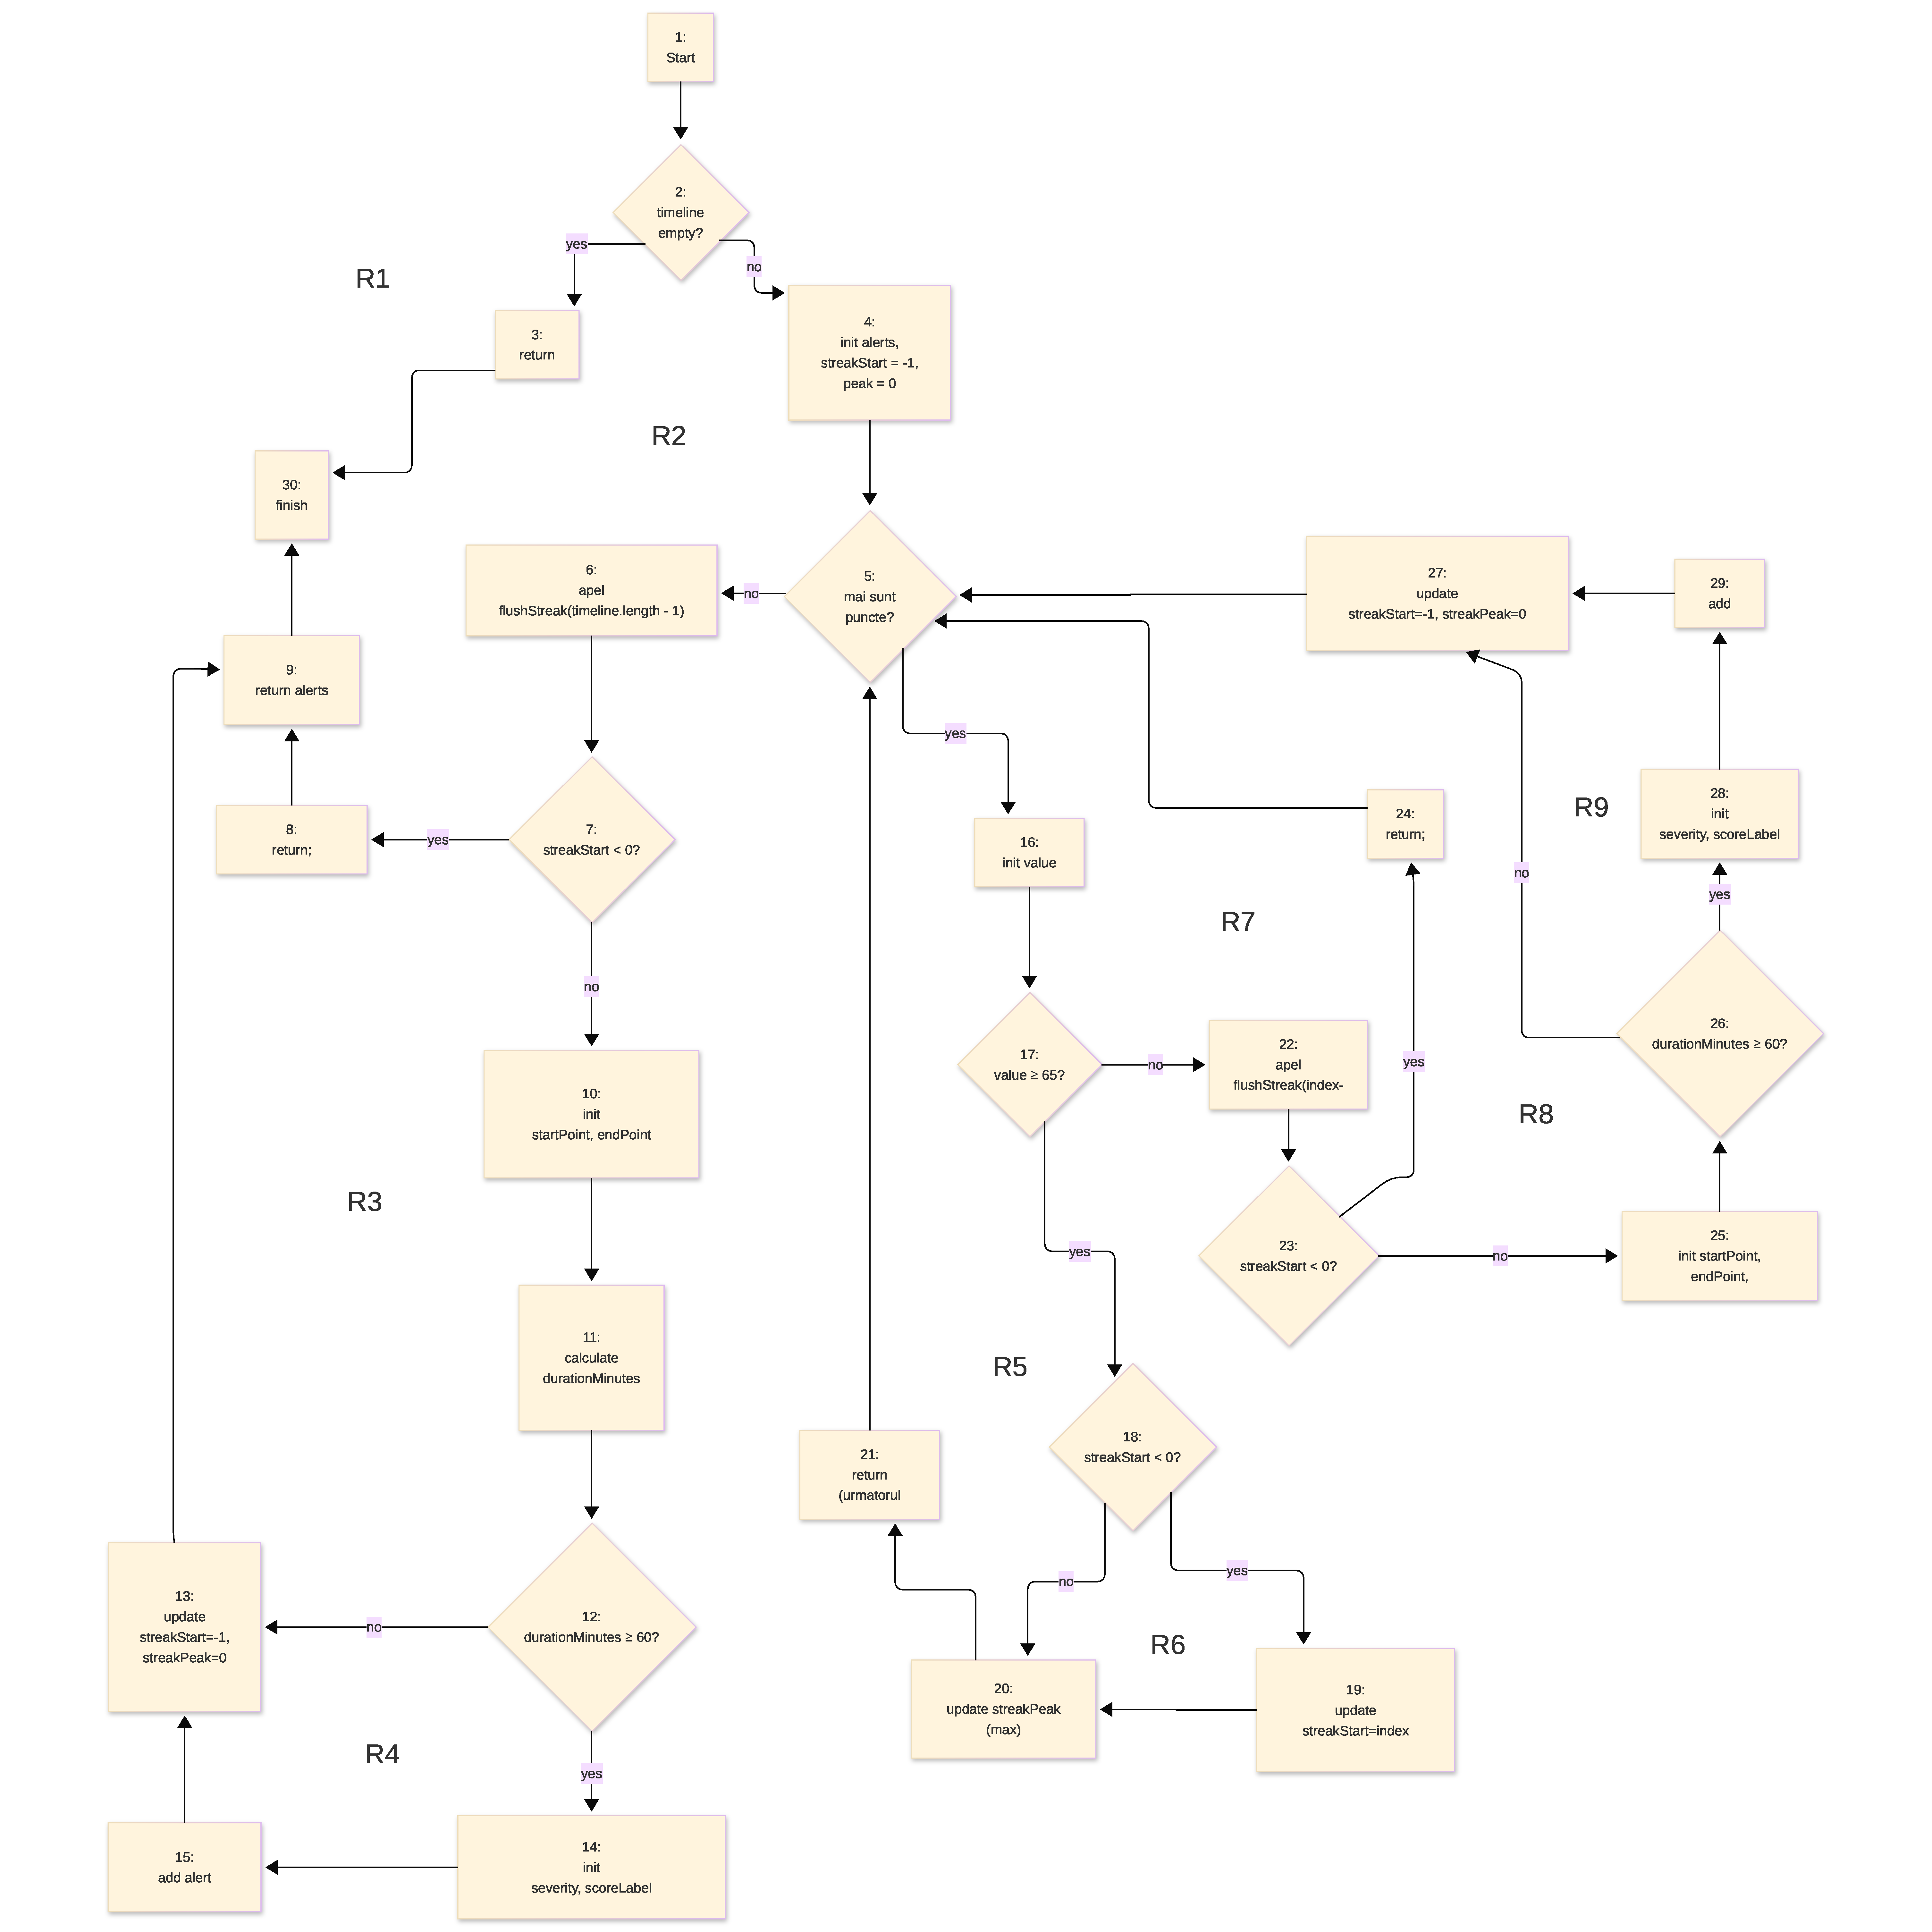
\includegraphics[width=0.97\textwidth]{figures/diagrams/cfg.pdf}
  \caption{CFG pentru \texttt{deriveProlongedAlert}.}
  \label{fig:cfg-derive-prolonged-alert}
\end{figure}

\noindent\textit{Nota:} pentru lizibilitate, apelul final \texttt{flushStreak(timeline.length - 1)} este comprimat in nodul \texttt{final flush}.

\subsubsection{Drumuri independente (set minim, CC=8)}
\begin{table}[htbp]
\centering
\footnotesize
\setlength{\tabcolsep}{5pt}
\renewcommand{\arraystretch}{1.15}
\begin{tabularx}{\textwidth}{p{0.9cm}p{3.6cm}p{4.9cm}X}
\toprule
\textbf{Path} & \textbf{Ramura noua acoperita} & \textbf{Date intrare (exemplu)} & \textbf{Rezultat asteptat} \\
\midrule
P1 & D1=True & \texttt{timeline=[]} & return lista vida, fara procesare. \\
P2 & D3=False + D5=True & toate valorile sub prag & fara alerta (nu exista streak activ). \\
P3 & D6=False & streak scurt (\(<60\) min) apoi intrerupere & fara alerta. \\
P4 & D6=True + D7=True & streak valid DISTRESS, durata \(\ge 60\) min & 1 alerta DISTRESS. \\
P5 & D6=True + D7=False & streak valid PAIN, durata \(\ge 60\) min & 1 alerta PAIN. \\
P6 & D4=False (streak continua) & mai multe puncte consecutive peste prag & streak mentinut corect, alerta unica la inchidere. \\
P7 & doua streak-uri mixte & primul \(<60\) min, al doilea \(\ge60\) min & exact 1 alerta (doar streak-ul valid). \\
P8 & inchidere prin \texttt{final flush} & streak activ la finalul listei & evaluare corecta la final (cu/fara alerta dupa durata). \\
\bottomrule
\end{tabularx}
\caption{Set compact de drumuri independente pentru acoperire basis-path.}
\label{tab:whitebox-compact-paths}
\end{table}

\section{Testarea de integrare}
\label{sec:testare-integrare}

\subsection{Scop}
Scopul testarii de integrare a fost validarea fluxului complet pentru endpoint-ul
\texttt{POST /api/doctor/patients/:patientId/readings}, de la nivel HTTP pana la nivel
controller/service si, in varianta extinsa, pana la persistenta reala in PostgreSQL.
S-au urmarit in special:
\begin{itemize}
  \item corectitudinea lantului \texttt{route -> middleware -> controller -> service};
  \item respectarea regulilor de autentificare si autorizare;
  \item persistenta corecta a citirilor emotionale;
  \item logica de alertare (creare alerta activa in scenarii de risc).
\end{itemize}

\subsection{Strategie}
Au fost implementate doua suite complementare:

\begin{itemize}
  \item \textbf{\texttt{doctor.readings.test.ts}}: integrare la nivel aplicatie (HTTP real prin \texttt{app}), cu infrastructura externa controlata prin mock (\texttt{Prisma}, \texttt{Influx}). Aceasta suita valideaza rapid fluxul functional si ramurile principale de business.
  \item \textbf{\texttt{doctor.readings.realdb.test.ts}}: integrare cu baza de date reala. Testul ruleaza pe schema dedicata \texttt{integration\_test}, aplica migrarile (\texttt{prisma migrate deploy}), face seed minim (\texttt{doctor/admin/ward/bed/patient}) si verifica efectiv datele scrise in PostgreSQL.
\end{itemize}

\subsection{Scenarii implementate}
\begin{table}[htbp]
\centering
\small
\setlength{\tabcolsep}{5pt}
\renewcommand{\arraystretch}{1.15}
\begin{tabularx}{\textwidth}{p{1.2cm}p{3.8cm}X p{2.0cm}}
\toprule
\textbf{ID} & \textbf{Suita} & \textbf{Scenariu} & \textbf{Rezultat} \\
\midrule
INT-01 & \texttt{doctor.readings.test.ts} &
Request fara header \texttt{Authorization} $\rightarrow$ raspuns \texttt{401}. &
Pass \\
INT-02 & \texttt{doctor.readings.test.ts} &
Token valid, dar rol \texttt{ADMIN} pe ruta de doctor $\rightarrow$ \texttt{403}. &
Pass \\
INT-03 & \texttt{doctor.readings.test.ts} &
Token \texttt{DOCTOR} valid + payload valid $\rightarrow$ \texttt{201}, apeluri corecte in service (\texttt{findUnique}, tranzactie, creare citire, logica alerta, apel Influx mock). &
Pass \\
\midrule
INT-04 & \texttt{doctor.readings.realdb.test.ts} &
Request fara \texttt{Authorization} in mediul cu DB real $\rightarrow$ \texttt{401}. &
Pass \\
INT-05 & \texttt{doctor.readings.realdb.test.ts} &
Token \texttt{ADMIN} pe ruta de doctor in mediul cu DB real $\rightarrow$ \texttt{403}. &
Pass \\
INT-06 & \texttt{doctor.readings.realdb.test.ts} &
Token \texttt{DOCTOR} valid + payload de risc ridicat $\rightarrow$ \texttt{201}; verificare in DB:
\texttt{EmotionReading} persistat + \texttt{PatientAlert} activ (tip \texttt{DISTRESS}, severitate corecta). &
Pass \\
\bottomrule
\end{tabularx}
\caption{Scenarii de integrare pentru endpoint-ul de readings.}
\label{tab:integration-readings}
\end{table}

\subsection{Mediu si executie}
Suita real-DB este controlata prin variabila de mediu \texttt{RUN\_DB\_INTEGRATION=1}.
Daca exista \texttt{DATABASE\_URL} in mediu, testul foloseste schema izolata
\texttt{integration\_test}; in lipsa acesteia, este prevazut fallback pe container PostgreSQL.

\noindent Comenzi de rulare:
\begin{verbatim}
# suita mock/full-app flow (rapid)
npm test --silent -- --runInBand --runTestsByPath src/__tests__/doctor.readings.test.ts

# suita cu baza reala (PowerShell)
$env:RUN_DB_INTEGRATION='1'
npm test --silent -- --runInBand --runTestsByPath src/__tests__/doctor.readings.realdb.test.ts
Remove-Item Env:RUN_DB_INTEGRATION
\end{verbatim}

\subsection{Rezultate obtinute}
La rularea curenta, ambele suite de integrare au trecut complet:
\begin{itemize}
  \item \texttt{doctor.readings.test.ts}: \textbf{3/3} teste trecute;
  \item \texttt{doctor.readings.realdb.test.ts}: \textbf{3/3} teste trecute;
  \item total integrare pe fluxul de readings: \textbf{6/6} teste trecute.
\end{itemize}

\subsection{Concluzie}
Prin combinarea suitei de integrare pe flux complet HTTP (cu dependinte externe controlate)
si a suitei de integrare cu persistenta reala, s-a obtinut un nivel bun de incredere asupra
functionalitatii endpoint-ului de readings: autentificarea/autorizarea, procesarea payload-ului,
persistenta datelor clinice si logica de alertare functioneaza corect in scenariile critice.


\section{Proiectare}
\subsection{Analiza cerințelor}
\subsection{Diagrama cazurilor de utilizare}
\subsection{Diagrame de interacțiune}
\section{Implementare}
\subsection{Server}
\subsection{Client}
\section{Testare}